\documentclass[12pt]{ruthesis}
\usepackage{amsmath}
\usepackage{amssymb}
\usepackage{latexsym}
\usepackage{subcaption} % for subfigures with separate captions
\usepackage{graphicx}
\usepackage{epsfig,epsf,rotating}
\usepackage{color}
\usepackage{epsf}

\usepackage{algorithm} % for the algorithm environment
\usepackage{algpseudocode} % for the algorithm environment

\usepackage{color} % For comments in color
\usepackage[normalem]{ulem} % For struck-out lines
\usepackage{footnote} % footnotes in text
%\usepackage{bracket} % expectation values
\usepackage[font={it}]{caption} % customizes the style of captions

\usepackage{theorem}
\newtheorem{proposition}{Proposition}

\theoremheaderfont{\itshape} {\theoremstyle{break}
\newtheorem{Fact}{Fact}[chapter]} \theoremstyle{break}
\newtheorem{Lem}{Lemma}[chapter] \theoremstyle{break}
\newtheorem{Thm}{Theorem}[chapter] {\theoremstyle{plain}
  \theorembodyfont{\rmfamily}  \newtheorem{Prf}{Proof}[chapter]}
{\theoremstyle{plain}
  \theorembodyfont{\rmfamily}  \newtheorem{Def}{Definition}[chapter]}

\usepackage{hyperref} % for interactive links. This always is loaded last
% new commands.
\algnewcommand{\LineComment}[1]{\State\(\triangleright\) #1}
% Comments for the whole line

\title{Tensor structured coupled cluster methods}

\author{Roman Schutski}
\department{Chemistry}
\school{Rice University}
\degree{Doctor of Philosophy}

\committee {
        Gustavo E. Scuseria, Chair \\
        Professor of Chemistry and Physics and Astronomy \and
        Anatoly Kolomeiski \\
        Professor of Chemistry\and
        Boris Yakobson\\
        Professor of Materials Science and NanoEngineering and Chemistry
}

\address{Houston, Texas}
\donemonth{Jan} \doneyear{2018} \makeindex
\begin{document}

  \begin{frontmatter}
   \pagenumbering{roman}
   %\makecover
   \maketitle
   \thispagestyle{empty}
\begin{abstract} 

A constant goal of quantum chemistry is devising accurate and computationally 
effective methods for molecular simulations. The accuracy of chemical 
predictions ultimately depends on the ability of a method to model electronic 
correlation for all ranges of parameters of the molecular systems. While 
effective tools exist, they often have unfavorable computational demands, are 
not systematically improvable or work well only in a particular region of 
molecular parameters, such as equilibrium geometry. In this thesis we present 
our work on two perspective approaches to capture electronic correlation with 
computational cost scaling only quartically in the system size.

First, we extend the application of the Projected Hartree-Fock (PHF)
method, which provides an effective description of electron correlation both 
near and far from the equilibrium. PHF is a simplest of a family of 
computational methods, which work effectively in the challenging to simulate 
strong correlation regime, while rigorously preserving physical symmetries of 
the solution. To make PHF usable for practical simulations, however, energy 
derivatives and dipole moments need to be evaluated. We derive analytical 
energy gradients for the single-reference PHF theory and use it to calculate 
equilibrium geometries and harmonic frequencies of sizable molecules.

%A way to systematically improve the PHF method is to increase the number of 
%reference states in the calculation. The resulting approach may reach exact 
%solution, but is much more demanding numerically. Fortunately, numerically 
%intensive parts of the multi-reference PHF can be effectively 
%parallelized on modern computers. We implemented parallel multi-reference PHF 
%and present simulations of very large Hubbard systems. 
 
Our second line of work is a family Coupled Cluster methods, often considered 
a "gold standard" of quantum chemistry. We show how to reduce the 
computational effort of the Restricted Coupled Cluster with Singles and 
Doubles by two orders of magnitude by introducing tensor decompositions. 
We demonstrate the accuracy of our low-cost approach by benchmark 
calculations on various organic molecules.

An interesting property of our new Tensor Structured Coupled Cluster is the 
ability to cure the failure of the original Coupled Cluster 
in strong correlation regime. We illustrate this by simulations of molecular 
dissociation and Hubbard systems. Lastly, we discuss the extension of our scheme 
to other methods in the Coupled Cluster family. 
 
\end{abstract}



   \section*{Acknowledgements}

I would thank my adviser Prof. Gustavo Scuseria for his guidance 
during the course of my graduate studies. His consistent support both in 
personal and academic aspects, as well as the atmosphere in his group shaped me 
as a researcher. 

During the years I was lucky to interact with Prof. Carlos 
Jim{\'e}nez-Hoyos, Dr. Ireneusz Bulik and Dr. Thomas Henderson,
who all taught me most of the important things to get started with the 
complicated craft of quantum chemistry. I am also grateful to Tom for reading 
and correcting multiple drafts of papers and manuscripts.

I would also thank Jinmo Zhao, Yiheng Qiu and Dr. Matthias Degroote for 
interesting discussions which started many ideas implemented in this work.
Special credit should go to Jinmo for his research on computer algebra 
systems, which made many projects possible, including this one.

Additionally, I would acknowledge Scuserians, including John Gomez, Dr. Jacob
Wahlen-Strothman, Dr. Kyle Throssell and others for making the group a great
place to work. My friends from Prof. Anatoly Kolomeisky's group, including 
Dr. Maria Kochugaeva and Dr. Alex Shvets, also contributed to make these 
years enjoyable.

During my graduate studies I was supported by The Department of Energy, award 
\# DE-SC0012575

Lastly, I am grateful to my family and my wife Irene for being a 
continuous source of inspiration and encouragement. Without their love and 
care this work would never be completed.
   \tableofcontents
   \listoffigures
   \listoftables
   \section*{Preface}

This thesis is based on some research I've done in Prof. Gustavo Scuseria group 
from 2012 to 2018, which resulted in following publications:

\begin{itemize}
 \item \emph{Multireference symmetry-projected variational approaches for 
ground and excited states of the one-dimensional Hubbard model}
R. Rodríguez-Guzmán, C. A. Jiménez-Hoyos, R. Schutski, G. E. Scuseria,
Phys. Rev. B \textbf{87} (23), 235129
 \item \emph{Analytic energy gradient for the projected Hartree–Fock method}
R. Schutski, C.A. Jiménez-Hoyos, G.E. Scuseria
J Chem. Phys. \textbf{140} (20), 204101
 \item \emph{Tensor-structured coupled cluster theory}
R. Schutski, J. Zhao, T. M. Henderson, G. E. Scuseria
J Chem. Phys. \textbf{147} (18), 184113 
\end{itemize}

Specific details are given in the chapters where these works are discussed. 
Parts of Chapter~\ref{ch:app_tcc} present research intended for subsequent 
publications.
  \end{frontmatter}
\pagenumbering{arabic}

\linespacing{1.7}

\chapter{Introduction
\label{ch:introduction}}
In recent 50 years electronic structure methods evolved into powerful tools 
used in many areas of research, including biochemistry, organic 
synthesis and catalysis, materials design and astrophysics.~\cite{} The 
electronic structure simulations help to understand many processes not easily 
accessible for experimental study, such as short-living transition complexes in 
chemical reactions, as well as to simulate exotic states of matter, such as 
superconductivity.~\cite{} An ever increasing demand for reliable 
simulations requires a constant increase of accuracy of existing tools, as 
well as the need to simulate larger and larger systems. 

Nowadays some successful approaches like density functional theory 
(DFT) or second order many-body perturbation theory (MP2) can be routinely used 
for the calculation of large size systems (200-1000 atoms). While being 
extremely efficient, these theories are often limited in their accuracy. 
Another problem of these efficient methods is their failure to 
describe many systems of interest, like transition states, open-shell molecules 
and states of matter caused by significant quantum effects, such as Mott 
insulators. The correlated behavior of electrons, which lays at the root of the 
description of challenging quantum systems, proved hard to be simulated in 
electronic structure. While a wide range of tools was developed over the 
years,~\cite{} they are still limited to small systems due to a very steep 
scaling of computational cost, and often suffer from numerical problems. Thus 
the search for effective methods capable to capture electron correlation at all 
ranges of molecular parameters remains an active topic of modern 
computational chemistry.

Traditional methods are based on configuration interaction (CI)-like expansion 
around the Hartree-Fock (HF) solution. Some of them, like the coupled cluster 
(CC) theory have evolved into highly efficient tools,\cite{benedict_intro} and 
their accuracy and robustness have been proven in many 
studies.\cite{benedict_intro} However, the steep scaling of computational cost 
limits the application of coupled cluster to small systems. The cost of the 
highly popular CCSD(T) method scales as $O(N^7)$, where $N$ is a measure of the 
systems size. This means that for a twice large system the effort to get 
solution is 128 times higher. The cause of the high cost of CC theories is a 
large number of optimization parameters they use, which scales as $O(N^6)$ for 
CCSD(T). This "curse of dimensionality" is a hallmark of methods based on 
orthogonal expansions around Hartree-Fock solutions.
Additionally, CC methods have difficulties at strong correlation when the HF 
solution becomes qualitatively incorrect. Alternative formulations of coupled 
cluster which used different reference functions~\cite{} have exponential 
scaling of computational cost and other numerical problems~\cite{} after decades 
of research.

However, there are many indications that traditional approaches are heavily 
overparameterized: the electron correlation in molecules decays as 
$\frac{1}{r^6}$, and hence the number of parameters should not grow 
exponentially, but rather linearly with the size of the system. One such 
indication is a family of recently developed Projected Hartree-Fock (PHF)
methods by Scuseria, Jim{\'e}nez-Hoyos and coworkers.~\cite{} In contrast to 
traditional approaches, PHF methods use a non-orthogonal expansion to 
parameterize the solution, while having a formal cost of the Hartree-Fock. While 
excelling at strong correlation, PHF methods, however, have a lower overall 
accuracy than coupled cluster approach. Merging the ideas of PHF and CC theories 
is an active topic of research.~\cite{}

This work pursues two related lines of research. First, we extend the 
application of the Projected Hartree-Fock for practical applications. The 
calculation of energy derivatives and dipole moments is often required in 
simulations, for example, to estimate equilibrium structure of molecules and 
their vibrational spectra. We derive analytical energy gradients for the 
single-reference PHF theory, which allows efficient calculation of the said 
quantities. Our development is supplied with exemplary calculations of 
some sizable molecules.

The second line of work is devoted to traditional coupled cluster 
methods. Coupled cluster parameterize the solution in terms of cluster 
amplitude tensors, the multidimensional arrays of numbers responsible for the 
implausible cost of CC methods. We show how to reduce the computational effort 
of the restricted coupled cluster with singles and doubles (RCCSD) by two 
orders of magnitude by introducing new representations for the cluster 
amplitudes. By using tensor decompositions high order amplitude tensors are 
approximated by sets of matrices, which is a key in reducing the cost of 
coupled cluster. We demonstrate the accuracy of our low-cost approach by 
benchmark calculations on various organic molecules. Lastly, we discuss other 
interesting interesting properties our approach may have.

In the next chapter a short review and theoretical background on the 
electronic structure problem is given. In 
chapter~\ref{ch:projected_hartree_fock} we provide a more in-depth 
overview of the Projected Hartree-Fock method, followed by the derivation of 
its energy gradient expression. We conclude with an example 
calculation of geometries and harmonic spectra of  benzine 
biradicals. In chapter~\ref{ch:tcc} we discuss the cause of high 
computational cost of CC methods, followed by the idea of tensor 
decompositions. Chapter~\ref{ch:tcc} is concluded with a derivation of a 
general scheme for applying tensor decompositions in context of coupled cluster 
methods. Chapter~\ref{ch:app_tcc} presents some applications of the proposed 
methods. We estimate the accuracy of approximating different ingredients of 
coupled cluster equations and test approximate CC methods on a large set of 
molecules. Chapter~\ref{ch:app_tcc} concludes with a discussion of an 
additional interesting properties our methods possess. An overall conclusion 
and outlook is given in chapter~\ref{ch:conclusions}.


\chapter{Preliminaries
\label{ch:preliminaries}}

\section{The electronic structure problem}
\label{sec:motivation}
The goal of quantum chemistry is to simulate and predict the behavior 
of chemical systems. At the root of chemical phenomena is a collective motion 
of electrons in the field of the nuclei. Together, electrons form a quantum 
many-body system. If one would be able to efficiently simulate the energy and 
the state of this system numerically, many questions of chemistry could be 
answered.

Since the advent of quantum mechanics all ingredients of many-body simulations 
are set. One needs to find the eigenvectors and eigenvalues of the 
Hamiltonian describing the system:
%
\begin{equation}
 H | \Psi \rangle = E | \Psi \rangle
 \label{eq:schroedinger}
\end{equation}
%
where $|\Psi \rangle = \Psi(\vec{x_{1}}, \vec{x_{2}}, \vec{x_{3}}\ldots 
\vec{x_{M}})$ is a wavefunction describing the state of an $M$-electron system 
and $E$ is the energy of the state. The variables $\vec{x}$ describe the 
degrees of freedom of the electrons, like coordinates and spin.
The Hamiltonian is usually written in a short form, due to the 
equivalence of quantum particles:
%
\begin{equation}
 \hat{H}(\vec{x^{\star}_{1}}\ldots 
\vec{x^{\star}_{M}}, \vec{x_{1}}\ldots 
\vec{x_{M}}) = h^{0} + \hat{h}(\vec{x^{\star}}, \vec{x}) + 
\frac{1}{2} \hat{V}(\vec{x^{\star}}, \vec{y^{\star}}, \vec{x}, 
\vec{y}) \qquad \forall \vec{x}, \vec{y} \in \{\vec{x}_{1}, \ldots, \vec{x}_{M} 
\}
\end{equation}
%
Here $h^{0}$ is a constant, $\hat{h}$ is a one-body part, e.g. it acts on each 
electron individually, and $\hat{V}$ is a two body part, acting on every pair 
of electrons. 

To solve~\ref{eq:schroedinger} in practice a discrete basis with $N$ 
functions is introduced for each of the variables $\vec{x}$, the procedure 
mathematicians would call Galerkin discretization. We denote this new 
$N$-valued discreet spaces by $\mathcal{V}$. As the number of basis functions 
increases, the solution of the discretized problem will approach the true 
solution of~\ref{eq:schroedinger}. After standard approximations, like a 
Born-Oppenheimer approximation,~\cite{} the molecular Hamiltonian becomes:
%
\begin{equation}
 \hat{H} = h^{nr} + h_{\mu \nu} a^{\dagger}_{\mu} a_{\nu} + \frac{1}{2} V_{\mu 
\nu \lambda \sigma} a^{\dagger}_{\mu} a^{\dagger}_{\nu} a_{\sigma} a_{\lambda}
\label{eq:hamiltonian}
\end{equation}
%
We imply summation over repeated indices in the expression above and the rest 
of the text unless otherwise stated. In Eqn.~\ref{eq:hamiltonian} the constant 
$h^{nr}$ is a nuclear repulsion energy, the one-body part $h$ describes a 
kinetic energy of an electron and its attraction to the nuclei:
%
\begin{equation}
 h_{\mu \nu} = \int d\vec{x_{1}} ~ \mu^{\star}(\vec{x_{1}}) \left( - 
\frac{1}{2} \nabla^2 - \sum_{a} \frac{Z_{a}}{|\vec{x_{1}} - 
\vec{r_{a}}|} \right) \nu(\vec{x_{1}})
\end{equation}
% 
The functions $\mu(\vec{x}), \nu(\vec{x})$ are basis functions used for the 
discretization of the problem and $r_{a}$ and $Z_{a}$ are the 
position and the charge of the nuclei. The two-body, or electron repulsion 
part, is
%
\begin{equation}
 V_{\mu \nu \lambda \sigma} = \int \int d\vec{x_{1}} d\vec{x_{2}}~ 
\mu^{\star}(\vec{x_{1}}) \nu^{\star}(\vec{x_{2}}) 
\frac{1}{|\vec{x_{1}} - \vec{x_{2}}|} 
\sigma(\vec{x_{2}}) \lambda(\vec{x_{1}}) 
\end{equation}
% 
We denoted by $a^{\dagger}_{\mu}$ and $a_{\mu}$ creation and 
annihilation operators. For example, $a^{\dagger}_{\mu}$ creates a single 
particle state $a^{\dagger}_{\mu} | - \rangle = | \mu \rangle$, where $| - 
\rangle$ is a physical vacuum. Equivalently, $a^{\dagger}_{\mu}$ and $a_{\mu}$ 
can be thought as simply a $\mu$-th unit vector (or its adjoint) in the 
discrete space $\mathcal{V}$, and $| - \rangle$  as a zero vector.

Despite a simple structure of the Hamiltonian, even a discretized
Schr{\"o}edinger equation is hard to solve. The solution is contained in an 
antisymmetric product (due to Pauli exclusion 
principle) of single particle vector spaces. The resulting space, called 
Hilbert space of the problem, is: 
%
\begin{equation}
 \mathcal{H} = \underbrace{\mathcal{V} \times \mathcal{V} \times \mathcal{V} 
\times \ldots}_{M ~\mathrm{times}}
\end{equation}
%
The Hamiltonian is thus a matrix in $\mathcal{H} \times \mathcal{H}$. The total 
size of the eigenvector of the Hamiltonian $|\Psi \rangle$ is 
of order of $N^{M}$ (it is actually $N \choose M$ because $\mathcal{H}$ is an 
antisymmetric vector space). Even for relatively small $M$ and $N$ a direct 
calculation of $|\Psi \rangle$ becomes prohibitive. The main problem of 
theoretical chemistry is thus, how to build feasible and accurate approximations 
to the true eigenvectors of $H$.

A commonly used approach is to use the variational principle~\cite{} to 
calculate the energy expectation value $\tilde{E}$ of a test wavefunction 
$\tilde{\Psi}$:
%
\begin{equation}
 \tilde{E} = \frac{\langle \tilde{\Psi} | H | \tilde{\Psi} \rangle}{\langle 
\tilde{\Psi} |\tilde{\Psi} \rangle} 
\end{equation}
%
It can be proved that this expectation value for a normalized  
function is an upper bound of the exact energy:
%
\begin{equation}
 E \geq E_{\mathrm{exact}}
\end{equation}
Although not all approaches to solve \ref{eq:schroedinger} are variational, 
variational nature is a valuable property of any particular method. 

\section{Solving Schr{\"o}edinger equation}
\label{sec:solving}
\subsection{Exact solution}
As we mentioned before, the direct solution of Sch{\"o}edinger equation is hard 
to obtain. One may still, however, embark on this task for very small systems. 
Let us introduce a basis of all states with $M$ electrons in the Hilbert 
space $\mathcal{H}$. This basis will contain all possible products of $M$ 
creation operators. Due to the antisymmetry of the 
wavefunction for electrons:
%
\begin{equation}
  \Psi(\vec{x_{1}}, \vec{x_{2}}) = - \Psi(\vec{x_{2}}, \vec{x_{1}}) 
\end{equation}
%
those products will contain only the combinations of $a^{\dagger}_{\mu}$ 
without repetitions over the index $\mu$ (repeated index will necessary turn 
product to zero):
%
\begin{equation}
 | \phi \rangle = \prod_{k=1}^{M} a^{\dagger}_{\mu_{k}} |- \rangle  
 \label{eq:slater_determinant}
\end{equation}
%
In total there will be $N \choose M$ products of the
form~\ref{eq:slater_determinant}, usually called Slater determinants or 
configurations. The Hamiltonian matrix can be written in this basis and 
diagonalized:
%
\begin{equation}
\begin{aligned}
 H_{ij} &= \langle \phi_{i} | \hat{H} | \phi_{j} \rangle \\
 | \Psi_{i} \rangle &= U_{ij} |\phi_{j} \rangle
\end{aligned}
\end{equation}
%
The eigenvectors $| \Psi \rangle$ obtained in this way and their respective 
eigenvalues are exact solutions to the Schr{\"o}edinger equation in a given 
basis. When available, they are often used as reference values in 
evaluation of the quality of quantum chemistry algorithms. Direct 
diagonalization, however, is possible only for the smallest systems. The 
simulation of a 12-electron system, like two carbon atoms, in a mediocre basis 
set of 10 basis functions per electron will involve a diagonalization of a 
matrix of size $1.054 \cdot 10^{16}$ which is already at the border of today's 
computational capabilities.

One may notice, however, that the molecular Hamiltonian is almost diagonal in 
the $M$-particle Hilbert space, as only one- and two-body parts are non-zero. 
This provides grounds for an important approximate method we are going to 
consider next. 

\subsection{Hartree-Fock solution}
The Hartree-Fock (HF) method is a starting point of most many-body approaches.
The idea of Hartree-Fock is to find a single best determinant to 
approximate the wavefunction:
%
\begin{equation}
 |\Psi_{SD} \rangle = \prod_{k=1}^{M} c_k^{\dagger} | -\rangle, \qquad 
c_{k}^{\dagger} = C_{\mu k} \cdot a^{\dagger}_{\mu}
\label{eq:single_determinant}
\end{equation}
% 
the parameters of this \emph{ansatz} are contained in the basis transformation 
matrix $C$. The energy 
of the state~\ref{eq:single_determinant} is:
%
\begin{equation}
 E = \frac{\langle \Psi_{SD} | H | \Psi_{SD} \rangle}{\langle \Psi_{SD} | 
\Psi_{SD} \rangle}
 \label{eq:hf_energy}
\end{equation}
%
The solution is found by minimizing the energy in~\ref{eq:hf_energy}, 
while constraining matrix $C$ to be unitary. The later is equivalent to 
minimizing a lagrangian:
%
\begin{equation}
\begin{aligned}
L(C, \epsilon) = h_{\mu \nu} \rho_{\nu \mu} &+ \frac{1}{2} 
V_{\mu \lambda \nu \sigma} \rho_{\nu \mu } \rho_{\sigma \lambda}  + 
\epsilon_{ij}(C^{\ast}_{\mu i} S_{\mu \nu} C_{\nu j} - 1_{N \times N})\\
\rho_{\nu \mu} &= C^{\ast}_{\mu i} C_{\nu i} 
\label{eq:hf_lagrangian}
\end{aligned}
\end{equation}
%
Here $C$ is a basis transformation one is solving for, $\epsilon$ is a 
set of lagrange multipliers used to enforce the unitary constraint, $1_{N 
\times N}$ is an identity matrix and $S_{\mu \nu} = \langle a^{\dagger}_{\mu} 
a_{\nu} \rangle $ is an overlap matrix of the possibly non-orthogonal original 
basis vectors $a$. Let us note that Hartree-Fock method 
is variational, and hence provides an upper bound for
the energy.\cite{levine2000quantum} 

There are multiple ways of solving Hartree-Fock equations, which we will not 
discuss here, but rather present a final result of the most well-known method 
of Roothaan.~\cite{roothan_carlos} By taking a derivative 
of~\ref{eq:hf_lagrangian} with respect to $C$, one ends up with a matrix 
equation:
%
\begin{equation}
\begin{aligned}
 FC^{\ast} &= \epsilon C^{\ast} S\\
 F_{\mu \nu} &= h_{\mu \nu} + V_{\mu \lambda \nu \sigma} \rho_{\sigma \lambda} 
 \label{eq:hf_roothaan}
\end{aligned}
\end{equation}
%
The equation~\ref{eq:hf_roothaan}, which looks like an eigenvalue problem for 
the Fock matrix $F$, is non-linear in $C$. It is solved by iterations starting 
from a guess for the transformation $C$. 

The Roothaans equation amounts to an important interpretation of the 
Hartree-Fock method. Note that if there would be no interaction term in the 
Hamiltonian, the Hartree-Fock would correspond to the exact 
diagonalization, and a Slater determinant, which is an antisymmetric direct 
product of single particle wavefunctions, would be an exact 
eigenstate. The Fock matrix in Eqn.~\ref{eq:hf_roothaan}, thus is a diagonal
approximation of the Hamiltonian, where the actual two-particle interaction 
$\hat{V}$ is replaced by a one-body term $\hat{V}_{eff} = \hat{V} \hat{\rho}$. 
The HF solution describes the electrons as if they would not immediately repel 
each other through Coulombic interaction, but rather move 
independently in an average potential $\hat{V}_{eff}$ of all other electrons. In 
reality, however, the electrons avoid each other dynamically. This brings us to 
the concept of electronic correlation: the true solution would need to account 
for the correlated motion of electrons. We would discuss this in more detail in 
the section.~\ref{sec:electronic_correlation} 

Overall, the Hartree-Fock method is a cornerstone of quantum chemistry due to 
its simplicity and theoretical basis. The computational cost of Hartree-Fock is 
$O(N^4)$ floating point operations in its simplest variants (and much less 
in optimized formulations\cite{}), which makes it one of the most 
affordable methods in electronic structure theory. Not being widely used on its 
own in practical simulations, it remains a usual starting point of most 
many-body approaches.


\subsection{Electronic correlation
\label{sec:electronic_correlation}}

Put simply, the electronic correlation is a difference between the exact and 
Hartree-Fock solution, and correlation energy is a difference between HF and 
exact energies. We will classify correlation based on two 
sources of errors introduced by the Hartree-Fock method, however, this division 
is only relative:

\begin{itemize}
\item Dynamic or weak correlation arises from small deviations of 
the Hartree-Fock potential and a faithful two-body interaction. It can be 
interpreted as an effect of short-range instantaneous repulsion between 
electrons.
\item Static or strong correlation emerges when the Hartree-Fock potential 
significantly deviates from the real two-body interaction, e.g. when the 
Hamiltonian is not a diagonally dominant matrix. Static correlation 
manifests as a near or exact degeneracy of different Slater determinants, and 
the single determinant picture becomes incorrect.
\end{itemize}

Let us illustrate the regions where different types of error of the HF method 
dominate in the process of nitrogen dissociation. 
%
\begin{figure}[tb]
%\includegraphics[width=\columnwidth]{figures/intro/n2_hf_exact}
\caption{Dissociation of nitrogen molecule using cc-pVDZ basis set. RHF refers 
to restricted Hartree-Fock, exact is taken from the exact diagonalization data.
\label{fig:n2_hf_exact}}
\end{figure}
%
Near the equilibrium the difference of Hartree-Fock and and exact energies is 
mostly related to short-range dynamical electronic repulsion. When the $N_2$ 
bond is stretched, the bonding, $\sigma^{\ast}_{2p}$ and antibonding $\pi_{2p}$ 
orbitals become degenerate, leading to the major overestimation of 
dissociation energy by the HF method. Let us now provide some examples of 
different types of correlation and its relation to physical phenomena.

Most correlation in "normal" systems is dynamical. Typical examples 
are usual organic molecules at equilibrium, most metals, semiconductors 
etc. Despite HF accounts for around $99\%$ of electronic energy, proper 
description of dynamical correlation is crucial in quantitative calculations.
For example, even for atoms, HF excitation energies may be wrong by 
more than as $40\%$~\cite{irek_9}, which leads to incorrect prediction of 
ionization potentials. Though difficult to generalize, lack of 
correlation leads to too short bonds at equilibrium, incorrect bond angles, 
errors in the dipole moments and too high harmonic vibrational 
frequencies.~\cite{irek_11, irek_12} HF usually predicts too high reaction 
barriers, which can be understood by the problems of HF to describe stretched 
bonds. Finally, Hartree-Fock approach is unable to predict pure 
dispersion interaction~\cite{irek_13}, correlation bound anions~\cite{irek_14} 
and similar systems.  

Statically correlated systems are where the shortcomings of Hartree-Fock theory 
are most pronounced, as independent particle picture becomes inappropriate. 
Static correlation is very common in extended systems and materials 
where $d$- and $f$-electron shells of atoms interact. Among many phenomena 
caused by strong correlation are large resistivity changes, huge volume changes 
across phase transitions, heavy fermion behavior, large 
magnetoresistence and high temperature superconductivity.~\cite{irek_15, 
irek_16}. Strongly correlated systems are of great importance and constant 
theoretical interest. Accounting for strong correlation is challenging for 
modern electronic structure methods.
 
The community of quantum chemists worked for decades to build methods to 
for properly accounting for electronic correlation. Up to now all existing 
approaches are flawed in one way or another. Nevertheless, let us list some 
important features an ideal approximate solution should have, which we will be 
using for comparison of different theories through the discussion:

\begin{itemize}
 \item Ideally, a theorist should seek an method which works well in the 
whole range of the parameters of the problem, e.g. which would provide accurate 
solutions both in strong and weak correlation regimes, independently of the 
size of the system. 

\item The method should be computationally tractable, with polynomial, and 
preferably low, dependence of cost on the system size.

\item A good many-body theory should be systematically improvable to provide a 
trade-off between accuracy and computational cost.

\item The method should be size consistent, which means that the energy of two 
non-interacting fragments $A$ and $B$ must be the sum of energies of those 
fragments calculated independently
\begin{equation}
 E(A \overset{d \longrightarrow \infty}{--} B) = E(A) + E(B)
\end{equation}

\item The predicted energy should scale linearly with the size of the system, 
e.g. the energy of $k$ non-interacting particles, like Helium atoms far apart 
from each other, should equal to the sum of energies of individual particles.
\begin{equation}
 E(k \cdot \mathrm{He}) = k \cdot E(\mathrm{He})
\end{equation}
This property is called size extensivity and is important in thermodynamics, 
where extensive quantities scale with system size
\end{itemize}

Let us now will provide more specific details on the coupled cluster 
and projected Hartree-Fock methods in the next chapters. 


%\chapter{Projected Hartree-Fock method
\label{ch:projected_hartree_fock}}
\section{Symmetry and degeneracy}

\section{Projected Hartree-Fock method and its gradients}

\section{Applications of PHF gradients}
\chapter{Preliminaries
\label{ch:preliminaries}}
In this section we will discuss the basic problem we're trying to solve.  
As this problem is generally computationally intractable, approximate solutions 
must be tried, and we will review those in Section~\ref{sec:approx_methods}. 
For certain special cases the exact solution is in fact available, and 
these constitute a valuable check on our approximations. We use one such 
special system, the one dimensional Hubbard model, in this work, and will 
briefly describe the model in \ref{sec:hubbard_hamiltonian}.

\section{The electronic structure problem}
\label{sec:motivation}
The goal of quantum chemistry is to simulate and predict the behavior 
of chemical systems. At the root of chemical phenomena is the motion 
of electrons in the field of the nuclei. Together, electrons form a quantum 
many-body system. If one could efficiently simulate the energy and 
the state of this system numerically, many questions of chemistry could be 
answered.

Since the advent of quantum mechanics all ingredients of many-body simulations 
are known. One needs to find the eigenvectors and eigenvalues of the 
Hamiltonian describing the system:
%
\begin{equation}
 \hat{H} | \Psi \rangle = E | \Psi \rangle
 \label{eq:schroedinger}
\end{equation}
%
where $\Psi(\vec{x_{1}}, \vec{x_{2}}, \vec{x_{3}}\ldots 
\vec{x_{M}}) = \langle \vec{x}_{1}, \vec{x}_{2}, \vec{x}_{2}, \ldots |\Psi 
\rangle$ is a wavefunction describing the state of an $M$-electron system 
and $E$ is the energy of the state. The variables $\vec{x}$ describe the 
degrees of freedom of the electrons, like coordinates and spin.
The Hamiltonian is usually written in a short form, due to the 
equivalence of quantum particles:
%
\begin{equation}
\begin{aligned}
 \hat{H} = h^{0} + \sum_{n} \hat{h}(\vec{x^{\star}_{n}}, \vec{x}_{n}) + 
\frac{1}{2} \sum_{n \neq m} \hat{V}(\vec{x^{\star}_{m}}, \vec{x^{\star}_{n}}, 
\vec{x}_{m}, 
\vec{x}_{n}) 
\end{aligned}
\end{equation}
%
Here $h^{0}$ is a constant, $\hat{h}$ is a one-body part, e.g. it acts on each 
electron individually, and $\hat{V}$ is a two body part, acting on every pair 
of electrons. 

To solve~\ref{eq:schroedinger} in practice a discrete basis with $N$ 
functions is introduced for each of the variables $\vec{x}$, the procedure 
mathematicians would call Galerkin discretization. We denote these new 
$N$-valued discrete spaces by $\mathcal{V}$. As the number of basis functions 
increases, the solution of the discretized problem will approach the true 
solution of~\ref{eq:schroedinger}. After standard approximations, like the 
Born-Oppenheimer approximation,~\cite{jensen2017introduction} the molecular 
Hamiltonian becomes:
%
\begin{equation}
 \hat{H} = h^{nr} + h_{\mu \nu} a^{\dagger}_{\mu} a_{\nu} + \frac{1}{2} V_{\mu 
\nu \lambda \sigma} a^{\dagger}_{\mu} a^{\dagger}_{\nu} a_{\sigma} a_{\lambda}
\label{eq:hamiltonian}
\end{equation}
%
We imply summation over repeated indices in the expression above and the rest 
of the text unless otherwise stated. In Eqn.~\ref{eq:hamiltonian} the constant 
$h^{nr}$ is the nuclear repulsion energy, the one-body part $h$ describes the 
kinetic energy of an electron and its attraction to the nuclei:
%
\begin{equation}
 h_{\mu \nu} = \int d\vec{x_{1}} ~ \mu^{\star}(\vec{x_{1}}) \left( - 
\frac{1}{2} \nabla^2 - \sum_{a} \frac{Z_{a}}{|\vec{x_{1}} - 
\vec{r_{a}}|} \right) \nu(\vec{x_{1}})
\end{equation}
% 
The functions $\mu(\vec{x}), \nu(\vec{x})$ are basis functions used for the 
discretization of the problem and $r_{a}$ and $Z_{a}$ are the 
position and the charge of the nuclei. The two-body, or electron repulsion 
part, is
%
\begin{equation}
 V_{\mu \nu \lambda \sigma} = \int \int d\vec{x_{1}} d\vec{x_{2}}~ 
\mu^{\star}(\vec{x_{1}}) \nu^{\star}(\vec{x_{2}}) 
\frac{1}{|\vec{x_{1}} - \vec{x_{2}}|} 
\sigma(\vec{x_{2}}) \lambda(\vec{x_{1}}) 
\end{equation}
% 
We denoted by $a^{\dagger}_{\mu}$ and $a_{\mu}$ creation and 
annihilation operators. For example, $a^{\dagger}_{\mu}$ creates a single 
particle state $a^{\dagger}_{\mu} | - \rangle = | \mu \rangle$, where $| - 
\rangle$ is the physical vacuum. Equivalently, $a^{\dagger}_{\mu}$ and 
$a_{\mu}$ can be thought as simply the $\mu$-th unit vector (or its adjoint) in 
the discrete space $\mathcal{V}$, and $| - \rangle$  as a zero vector.

Despite the simple structure of the Hamiltonian, even a discretized
Schr{\"o}dinger equation is hard to solve. The solution is contained in an 
antisymmetric product (due to the Pauli exclusion 
principle) of single particle vector spaces. The resulting space, called 
the Hilbert space of the problem, is: 
%
\begin{equation}
 \mathcal{H} = \underbrace{\mathcal{V} \times \mathcal{V} \times \mathcal{V} 
\times \ldots}_{M ~\mathrm{times}}
\end{equation}
%
The Hamiltonian is thus a matrix in $\mathcal{H} \times \mathcal{H}$. The total 
size of the eigenvector of the Hamiltonian $|\Psi \rangle$ is 
on the order of $N^{M}$ (it is actually $N \choose M$ because $\mathcal{H}$ is 
an antisymmetric vector space). Even for relatively small $M$ and $N$ a direct 
calculation of $|\Psi \rangle$ becomes prohibitive. The main problem of 
theoretical chemistry is how to build feasible and accurate 
approximations to the true eigenvectors of $H$.

A commonly used approach is to use the variational 
principle~\cite{jensen2017introduction} to 
calculate the energy expectation value $\tilde{E}$ of a test wavefunction 
$\tilde{\Psi}$:
%
\begin{equation}
 \tilde{E} = \frac{\langle \tilde{\Psi} | H | \tilde{\Psi} \rangle}{\langle 
\tilde{\Psi} |\tilde{\Psi} \rangle} 
\end{equation}
%
It can be proven~\cite{levine2000quantum} that this expectation value for a 
normalizable function is an upper bound of the exact energy:
%
\begin{equation}
 E \geq E_{\mathrm{exact}}
\end{equation}
Although not all approaches to solve \ref{eq:schroedinger} are variational, 
variational nature is a valuable property of any particular method. 

\section{Solving the Schr{\"o}dinger equation}
\label{sec:solving}
\subsection{Exact solution}
As we mentioned before, the direct solution of the Sch{\"o}dinger equation is 
hard to obtain. One may still, however, embark on this task for very small 
systems. Let us introduce a basis of all states with $M$ electrons in the 
Hilbert space $\mathcal{H}$. This basis will contain all possible products of 
$M$ creation operators. Due to the antisymmetry of the 
wavefunction for electrons:
%
\begin{equation}
  \Psi(\vec{x_{1}}, \vec{x_{2}}) = - \Psi(\vec{x_{2}}, \vec{x_{1}}) 
\end{equation}
%
those products will contain only the combinations of $a^{\dagger}_{\mu}$ 
without repetitions over the index $\mu$ (a repeated index will necessarily 
turn the product to zero):
%
\begin{equation}
 | \phi \rangle = \prod_{k=1}^{M} a^{\dagger}_{\mu_{k}} |- \rangle  
 \label{eq:slater_determinant}
\end{equation}
%
In total there will be $N \choose M$ products of the
form~\ref{eq:slater_determinant}, usually called Slater determinants or 
configurations. The Hamiltonian matrix can be written in this basis and 
diagonalized:
%
\begin{equation}
\begin{aligned}
 H_{ij} &= \langle \phi_{i} | \hat{H} | \phi_{j} \rangle \\
 | \Psi_{i} \rangle &= U_{ij} |\phi_{j} \rangle
\end{aligned}
\end{equation}
%
The eigenvectors $| \Psi \rangle$ obtained in this way and their respective 
eigenvalues are exact solutions to the Schr{\"o}dinger equation in a given 
basis. When available, they are often used as reference values in the
evaluation of the quality of quantum chemistry algorithms. Direct 
diagonalization, however, is possible only for the smallest systems. The 
simulation of a 12-electron system, such as two carbon atoms, in a mediocre 
basis set of 10 basis functions per electron will involve diagonalization of 
a matrix of size $1.054 \cdot 10^{16}$ which is already at the border of 
today's computational capabilities.

One may notice, however, that the molecular Hamiltonian is almost diagonal in 
the $M$-particle Hilbert space, as only one- and two-body parts are non-zero. 
This provides grounds for an important approximate method we are going to 
consider next. 

\subsection{Hartree-Fock solution}
The Hartree-Fock (HF) method is the starting point of most many-body approaches.
The idea of Hartree-Fock is to find a single best determinant to 
approximate the wavefunction:
%
\begin{equation}
 |\Psi_{SD} \rangle = \prod_{k=1}^{M} c_k^{\dagger} | -\rangle, \qquad 
c_{k}^{\dagger} = C_{\mu k} \cdot a^{\dagger}_{\mu}
\label{eq:single_determinant}
\end{equation}
% 
The parameters of this \emph{ansatz} are contained in the basis transformation 
matrix $C$. The energy 
of the state~\ref{eq:single_determinant} is:
%
\begin{equation}
 E = \frac{\langle \Psi_{SD} | H | \Psi_{SD} \rangle}{\langle \Psi_{SD} | 
\Psi_{SD} \rangle}
 \label{eq:hf_energy}
\end{equation}
%
The solution is found by minimizing the energy in~\ref{eq:hf_energy}, 
while constraining matrix $C$ to be unitary. The later is equivalent to 
minimizing a Lagrangian:
%
\begin{equation}
\begin{aligned}
L(C, \epsilon) = h_{\mu \nu} \rho_{\nu \mu} &+ \frac{1}{2} 
V_{\mu \lambda \nu \sigma} \rho_{\nu \mu } \rho_{\sigma \lambda}  + 
\epsilon_{ij}(C^{\ast}_{\mu i} S_{\mu \nu} C_{\nu j} - 1_{N \times N})\\
\rho_{\nu \mu} &= C^{\ast}_{\mu i} C_{\nu i} 
\label{eq:hf_lagrangian}
\end{aligned}
\end{equation}
%
Here $C$ is the basis transformation one is solving for, $\epsilon$ is a 
set of Lagrange multipliers used to enforce the unitary constraint, $1_{N 
\times N}$ is the identity matrix and $S_{\mu \nu} = \langle a^{\dagger}_{\mu} 
a_{\nu} \rangle $ is an overlap matrix of the possibly non-orthogonal original 
basis vectors $a$. Let us note that the Hartree-Fock method 
is variational, and hence provides an upper bound for
the energy.\cite{levine2000quantum} 

There are multiple ways of solving the Hartree-Fock equations, which we will 
not discuss here, but rather present a final result of the most well-known 
method of Roothaan.~\cite{roothaan1951new} By taking the derivative 
of~\ref{eq:hf_lagrangian} with respect to $C$, one ends up with a matrix 
equation:
%
\begin{equation}
\begin{aligned}
 FC^{\ast} &=  C^{\ast} S \epsilon\\
 F_{\mu \nu} &= h_{\mu \nu} + V_{\mu \lambda \nu \sigma} \rho_{\sigma \lambda} 
 \label{eq:hf_roothaan}
\end{aligned}
\end{equation}
%
Equation~\ref{eq:hf_roothaan}, which looks like an eigenvalue problem for 
the Fock matrix $F$, is non-linear in $C$. It is solved by iteration starting 
from a guess for the transformation $C$. At convergence the matrix $C$ presents 
a transformation from the atomic orbital (AO) to molecular orbital (MO) basis. 
The Fock matrix in the MO basis is diagonal, and its diagonal elements can be 
interpreted as single particle energy levels. 

Roothaan's equation amounts to an important interpretation of the 
Hartree-Fock method. Note that if there would be no interaction term in the 
Hamiltonian, the Hartree-Fock would correspond to the exact 
diagonalization, and a Slater determinant, which is an antisymmetric direct 
product of single particle wavefunctions, would be an exact 
eigenstate. The Fock matrix in Eqn.~\ref{eq:hf_roothaan}, thus is a diagonal
approximation of the Hamiltonian, where the actual two-particle interaction 
$\hat{V}$ is replaced by a one-body term $\hat{V}_{eff} = \hat{V} \hat{\rho}$. 
The HF solution describes the electrons as if they would not immediately repel 
each other through Coulombic interaction, but rather move 
independently in an average potential $\hat{V}_{eff}$ of all other electrons. 
In reality, however, the electrons avoid each other dynamically. This brings us 
to the concept of electronic correlation: the true solution would need to 
account for the correlated motion of electrons. We will discuss this in more 
detail in the next section.

Overall, the Hartree-Fock method is a cornerstone of quantum chemistry due to 
its simplicity and theoretical basis. The computational cost of Hartree-Fock is 
$O(N^4)$ floating point operations in its simplest variants (and much less 
in optimized formulations\cite{goedecker1999linear}), which makes it one of the 
most affordable methods in electronic structure theory. Despite not being 
widely used on its own in practical simulations, it remains a usual starting 
point of most many-body approaches.


\subsection{Electronic correlation
\label{sec:electronic_correlation}}

Put simply, electronic correlation is the difference between the exact and 
Hartree-Fock solution, and the correlation energy is the difference between 
the HF and exact energies. We will classify correlation based on two 
sources of errors introduced by the Hartree-Fock method; however, this division 
is only relative:

\begin{itemize}
\item Dynamic or weak correlation arises from small deviations of 
the Hartree-Fock potential from the faithful two-body interaction. It can be 
interpreted as an effect of short-range instantaneous repulsion between 
electrons.
\item Static or strong correlation emerges when the Hartree-Fock potential 
significantly deviates from the real two-body interaction, e.g. when the 
Hamiltonian is not a diagonally dominant matrix. Static correlation 
manifests as a near or exact degeneracy of different Slater determinants, and 
the single determinant picture becomes incorrect.
\end{itemize}

Let us illustrate the regions where different types of error of the HF method 
dominate in the process of nitrogen dissociation. 
%
\begin{figure}[tb]
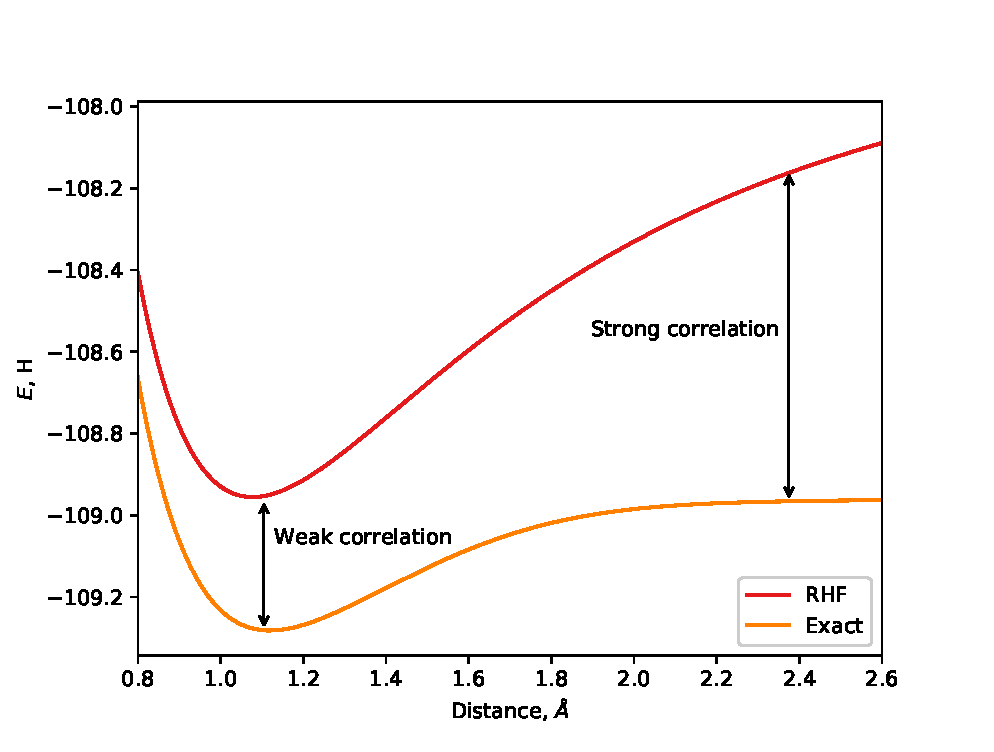
\includegraphics[width=\columnwidth]{figures/prelim/hf_exact}
\caption{Regions of weak and strong correlation along the dissociation 
curve of the nitrogen molecule. RHF refers to restricted Hartree-Fock, exact is 
taken from the exact diagonalization data.
\label{fig:n2_hf_exact}}
\end{figure}
%
Near equilibrium the difference of Hartree-Fock and and exact energies is 
mostly related to short-range dynamical electronic repulsion. When the 
bond is stretched, the bonding, $\sigma^{\ast}_{2p}$ and $\pi_{2p}$ 
orbitals become degenerate, as well as antibonding $\sigma^{\ast}_{2p}$ and 
$\pi_{2p}$ orbitals. Finally, at infinite distance all $2p$ orbitals are the 
same, which leads to the major overestimation of dissociation energy by the HF 
method. Let us now provide some examples of different types of correlation and 
its relation to physical phenomena.

Most correlation in "normal" systems is dynamical. Typical examples 
are usual organic molecules at equilibrium, most metals, semiconductors 
etc. While HF accounts for around $99\%$ of electronic energy, proper 
description of dynamical correlation is crucial in quantitative calculations.
For example, even for atoms, HF excitation energies may be wrong by 
more than $40\%$~\cite{wilson2013methods}, which leads to incorrect prediction 
of ionization potentials. The lack of correlation leads to too short bonds at 
equilibrium, incorrect bond angles, errors in the dipole moments and too high 
harmonic vibrational frequencies.~\cite{helgaker2014molecular, 
scott1996harmonic} HF usually predicts too high reaction barriers, which can be 
understood by the inability of HF to describe stretched bonds. Finally, the 
Hartree-Fock approach is unable to predict pure dispersion 
interaction, correlation bound anions~\cite{voora2013existence} and similar 
systems.

Statically correlated systems are where the shortcomings of Hartree-Fock theory 
are most pronounced, as the independent particle picture becomes inappropriate. 
Static correlation is very common in extended systems and materials 
where $d$- and $f$-electron shells of atoms interact. Among many phenomena 
caused by strong correlation are large resistivity changes, huge volume changes 
across phase transitions, heavy fermion behavior, large 
magnetoresistence and high temperature superconductivity.~\cite{imada1998metal, 
kotliar2004strongly}. Strongly correlated systems are of great importance and 
constant theoretical interest. Accounting for strong correlation is challenging 
for modern electronic structure methods.

As we hope the reader is convinced, the proper description of electronic 
correlation is essential for quantitative many-body simulations. We should now 
follow with the discussion of the approximate many-body methods.

\section{Approximate many-body methods
\label{sec:approx_methods}}
\subsection{Configuration expansion}
As an exact solution of the Schr{\"o}dinger equation can be obtained by 
diagonalizing the Hamiltonian in the basis of all possible determinants, one 
may try to do it over a subset of configurations to save on numerical cost. 
On the other hand, the HF solution $|\Phi_{0}\rangle$ is the best single 
determinant representation of the wavefunction. A natural idea is then to build 
a subset of configurations which are close to $|\Psi_{0}\rangle$:
%
\begin{equation}
\begin{aligned}
 |\Psi \rangle &= u_{0} |\Psi_{0}\rangle + u_{i}^{a} 
c^{\dagger}_{a} c_{i} |\Psi_{0}\rangle + u_{ij}^{ab} c^{\dagger}_{a} 
c^{\dagger}_{b} c_{j} c_{i} |\Psi_{0}\rangle + u_{ijk}^{abc} 
c^{\dagger}_{a} c^{\dagger}_{b} c^{\dagger}_{c} c_{k} c_{j} c_{i} 
|\Psi_{0}\rangle + \ldots \\
 &= \hat{U}_{0} |\Psi_{0}\rangle + \hat{U}_{1} |\Psi_{0}\rangle + \hat{U}_{2} 
|\Psi_{0}\rangle + \hat{U}_{3} 
|\Psi_{0}\rangle \ldots
\end{aligned}
\label{eq:ci_expansion}
\end{equation}
%
Here expansion coefficients $u$ are used for the different orders of 
substituted determinants. We denote occupied HF states by indices 
$i,j,k,\ldots$ and unocupied states by $a,b,c,\ldots$. Note that because 
operators $c$ act in an orthogonal HF basis, all of the terms 
in~\ref{eq:ci_expansion} represent orthogonal configurations. 
Expansion~\ref{eq:ci_expansion} is the basis of many traditional many body 
methods, the simplest example being the Configuration Interaction (CI) method. 
By taking the expectation value of the Hamiltonian with $|\Psi\rangle$ 
and applying the linear variational theorem one ends up with an eigenvalue 
problem for the coefficients $U$:
%
\begin{equation}
 HU = EU
 \label{eq:ci_eigenvalue}
\end{equation}
%
The solution to the above equation provides a variational estimate of 
the energy. It is evident that when all substitutions in $|\Phi_{0}\rangle$ are 
taken we would return to the exact diagonalization, or the full 
configuration interaction (FCI) problem. To make the computation affordable,the 
expansion~\ref{eq:ci_expansion} is usually truncated at double excitations:
%
\begin{equation}
 |\Psi \rangle = u_{0} |\Psi_{0}\rangle + u_{i}^{a} 
c^{\dagger}_{a} c_{i} |\Psi_{0}\rangle + u_{ij}^{ab} c^{\dagger}_{a} 
c^{\dagger}_{b} c_{j} c_{i} |\Psi_{0}\rangle
\end{equation}
%
Truncated CI methods are not very popular in modern calculations. 
Nevertheless, they are used sometimes if excited states are of interest 
and excitation energies need to be 
calculated.~\cite{sherrill1999configuration,head1994doubles}
The problem with the truncated CI approach is that it is neither size 
consistent nor size extensive.~\cite{helgaker2014molecular, 
jensen2017introduction} 

A method is size consistent~\cite{pople1976theoretical} if the energy of two 
non-interacting fragments $A$ and $B$ is the sum of the energies of those 
fragments calculated independently
\begin{equation}
 E(A \overset{d \longrightarrow \infty}{-} B) = E(A) + E(B)
\end{equation}

Size extensivity means that the energy scales linearly with the size of the 
system. For example, the energy of $k$ interacting fragments, such as Helium 
atoms far apart from each other, should equal to the sum of energies of 
individual fragments.
\begin{equation}
 E(k \cdot \mathrm{He}) = k \cdot E(\mathrm{He})
\end{equation}
In thermodynamics extensive quantities scale with the system 
size,~\cite{bartlett1978many} therefore size extensivity is a desirable 
property of any many-body approach.

It turns out that there is a better way of parameterizing the wavefunction in 
the form~\ref{eq:ci_expansion}, which eliminates the drawbacks of CI. This way 
is provided by the coupled cluster ansatz.

\subsection{Coupled Cluster theory}
Since its introduction in nuclear physics,\cite{coester1958bound, 
coester1960short} coupled cluster has become highly popular in quantum 
chemistry due to its exceptional ability to capture weak electronic 
correlation, while still having polynomial computational cost in the size of 
the basis. Another attractive property of CC theory is that while having the 
same number of parameters as CI methods, CC methods are size consistent and 
size extensive\footnote{Coupled cluster is size 
extensive and size consistent only when the reference 
wavefunction has these properties. For example, 
restricted HF-based coupled cluster is not extensive nor consistent in a case 
when an even number of electrons is split into two fragments with an odd number 
of electrons.}, \cite{pople1978electron, 
bartlett1978many, crawford2000introduction, bartlett2007coupled}. In coupled 
cluster the wavefunction is parameterized with an exponential ansatz:
%
\begin{equation}
 |\Psi\rangle = e^{\hat{T}} |\Psi_{0}\rangle
 \label{eq:cc_ansatz}
\end{equation}
Here the excitation operator $\hat{T}$ acts on a reference wavefunction 
$|\Psi_{0}\rangle$ (usually a Hartree-Fock determinant). The excitation 
operator has the same form as in case of CI:
%
\begin{equation}
\begin{aligned}
 \hat{T} &= {}^1\hat{T} + {}^2\hat{T} + {}^3\hat{T} + \ldots \\ 
 &= {}^{1}T_{i}^{a} c^{\dagger}_{a} c_{i} + \frac{1}{4} {}^2T_{ij}^{ab} 
c^{\dagger}_{a} c^{\dagger}_{b} c_{j} c_{i} + \frac{1}{36} {}^3T_{ijk}^{ab} 
c^{\dagger}_{a} c^{\dagger}_{b} c^{\dagger}_{c} c_{k} c_{j} c_{i} 
+\ldots
\end{aligned}
\end{equation}
The coefficient tensors $T$ are called cluster amplitudes. An excitation 
operator of order $n$ is defined by the following expression:
%
\begin{equation}
 {}^{n}\hat{T} = \frac{1}{(n!)^2}{}^{n}T_{ijk\ldots}^{abc\ldots} 
c^{\dagger}_{a} c^{\dagger}_{b} c^{\dagger}_{c} \ldots c_{k} c_{j} 
c_{i} 
\end{equation}
%
The exponential of the excitation operator is understood in terms of a 
polynomial series. Note that in contrast with CI, this ansatz contains not only 
linear excitations, but also products of excitations:
%
\begin{equation}
\begin{aligned}
  & e^{\hat{T}} |\Psi_{0}\rangle = \\
  & (1 + \hat{T} + \frac{1}{2} \hat{T}^{2} + \frac{1}{6} \hat{T}^3 + \ldots) | 
\Psi_{0} \rangle = \\
  & (1 + {}^{1}\hat{T} + \frac{1}{2}({}^{1}\hat{T})^{2} + \ldots + \\
  & {}^{2}\hat{T} + \frac{1}{2}({}^{2}\hat{T})^{2} + \ldots + \\
  & ({}^{1}\hat{T}) ({}^{2}\hat{T}) + \frac{1}{2}({}^{1}\hat{T})^{2} 
({}^{2}\hat{T}) + \ldots) |\Psi_{0} \rangle \\
\end{aligned}
\end{equation}
%
The size extensivity of coupled cluster is a direct consequence of the 
product terms occuring in the exponential function. 

The energy expression can be obtained by inserting~\ref{eq:cc_ansatz} into the 
Schr{\"o}dinger equation:
%
\begin{equation}
 \hat{H} e^{\hat{T}} | \Psi_{0} \rangle  = E |\Psi_{0} \rangle
 \label{eq:half_cc_schroedinger}
\end{equation}
%
This equation, however, can not be solved variationally with low 
cost. The expectation value would be:
%
\begin{equation}
 \frac{\langle \Psi_{0} | e^{\hat{T}^{\dagger}} \hat{H} e^{\hat{T}} | \Psi_{0} 
\rangle}{\langle \Psi_{0} | e^{\hat{T}^{\dagger}} e^{\hat{T}} |\Psi_{0} 
\rangle} = E 
\end{equation}
%
The variational expression above contains all possible excitations up to the 
number of electrons $M$ and no natural truncation scheme exists. 
Solving~\ref{eq:half_cc_schroedinger} variationally thus may not be easier 
than solving the FCI problem. Alternatively, 
Equation~\ref{eq:half_cc_schroedinger} can be solved projectively by 
multiplying it from the left by $e^{-\hat{T}}$:
%
\begin{equation}
 e^{-\hat{T}} \hat{H} e^{\hat{T}} |\Psi_{0} \rangle = E | \Psi_{0} \rangle
\end{equation}
%
The similarity transformed Hamiltonian $\bar{H} = e^{-\hat{T}} \hat{H} 
e^{\hat{T}}$ can be significantly simplified by using 
the Baker-Campbell-Hausdorf (BCH) expansion~\cite{crawford2000introduction, 
shavitt2009many}, which leads 
to nested commutators of the amplitudes and the Hamiltonian:
%
\begin{equation}
\begin{aligned}
  &e^{-\hat{T}} \hat{H} e^{\hat{T}} = \hat{H} + \left[ \hat{H}, \hat{T} \right] 
+ \frac{1}{2!} \left[ \left[ \hat{H}, \hat{T} \right], \hat{T} \right] +\\
&\frac{1}{3!} \left[ \left[ \left[  \hat{H}, \hat{T} \right], \hat{T} \right], 
\hat{T} \right] + \frac{1}{4!} \left[ \left[ \left[ \left[ \hat{H}, \hat{T} 
\right], \hat{T} \right], \hat{T} \right], \hat{T} \right] + \ldots
\end{aligned}
\label{eq:bch_expansion}
\end{equation}
%
Here $\left[ \hat{H}, \hat{T} \right] = \hat{H} \hat{T} - \hat{T}\hat{H}$.
To evaluate the BCH expansion one needs to start with the Hamiltonian in the 
HF basis. The transformation of the Hamiltonian to the mean field basis can 
be done by using operator algebra (see, for example 
Ref.~\cite{crawford2000introduction} for a complete derivation of this 
expression):
%
\begin{equation}
 \hat{H} = E_{0} + F_{q}^{p} c^{\dagger}_{p} c_{q} + \frac{1}{4} (V_{rs}^{pq} 
- V_{sr}^{pq}) c^{\dagger}_{p} c^{\dagger}_{q} c_{r} c_{s}
\end{equation}
%
Here $E_{0}$ is the Hartree-Fock energy, $F$ is a Fock matrix 
(see~\ref{eq:hf_roothaan}), and $V$ is the two electron interaction in the 
molecular orbital basis. The indices $p,q,r,s,\ldots$ in the Hamiltonian are 
general indices, e.g. they run over both occupied and virtual spaces.

By using the commutator arithmetic~\cite{shavitt2009many} it can be shown that 
each commutator between $\hat{H}$ and $\hat{T}$ transforms one general index 
of the Hamiltonian into a Kronecker delta function. As the Hamiltonian has only 
four different general operators, there can only be four commutators with 
$\hat{T}$, and the BCH expansion naturally truncates after the fifth term in 
Eqn.~\ref{eq:bch_expansion}. The similarity transformed Hamiltonian $\bar{H}$ 
will thus be a polynomial of up to fourth order in excitation operators 
$\hat{T}$.

If the excitation operator $\hat{T}$ contained all possible orders of 
excitations~$\{ {}^{1}\hat{T}, {}^{2}\hat{T}, \ldots \}$, 
the coupled cluster would be equivalent to exact diagonalization. To have a 
practical method one needs to truncate $\hat{T}$. The most common 
truncation level is doubles, e.g:
%
\begin{equation}
 \hat{T} =  {}^{1}T_{i}^{a} c^{\dagger}_{a} c_{i} + \frac{1}{4} {}^2T_{ij}^{ab} 
c^{\dagger}_{a} c^{\dagger}_{b} c_{j} c_{i}
\end{equation}
%
The order of excitation operator $\hat{T}$ determines the name of a particular 
coupled cluster method, with \textbf{S} meaning singles, \textbf{D} denoting 
doubles, \textbf{T} referring to triples etc. Note that by construction CCSD is 
exact for 2-electron systems, CCSDT is exact for 3-electron systems and so on. 
The effect of including single excitations on the accuracy of coupled cluster 
is usually not large, and hence they can often be omitted resulting in the 
simpler coupled cluster with doubles (CCD) method. The cost of coupled cluster 
rises quickly with the order of excitation operator, being of order $O(N^6)$ 
for CCSD, $O(N^8)$ for CCSDT and $O(N^{10})$ for CCSDTQ (see 
chapter~\ref{ch:tcc} for a detailed discussion).

After using the BCH expansion, we are finally in a position to formulate a 
general coupled cluster method. The similarity transformed Schr{\"o}dinger 
equation is:
%
\begin{equation}
 e^{-\hat{T}} \hat{H} e^{\hat{T}} |\Psi_{0}\rangle = E |\Psi_{0}\rangle
 \label{eq:sim_cc_schroedinger}
\end{equation}
It is obvious that the energy can be extracted by taking an expectation value 
with $\langle \Psi_{0}|$. The energy equation is:
%
\begin{equation}
 E = \langle \Psi_{0} | \bar{H} | \Psi_{0} \rangle
 \label{eq:cc_energy}
\end{equation}
The energy expression contains only single (if present in the excitation 
operator $\hat{T}$) and double excitations. Higher orders of 
excitation operator can not be compensated by the Hamiltonian, and would 
necessarily produce orthogonal configurations on the left and right hand sides 
of the expectation value in~\ref{eq:cc_energy}. By using these Slater-Condon 
rules~\cite{jensen2017introduction} the energy of coupled cluster is:
%
\begin{equation}
\begin{aligned}
 E &= \langle \Psi_{0} | (1 - {}^{1}\hat{T} - {}^{2}\hat{T} + \ldots) H (1 + 
{}^{1}\hat{T} + \frac{1}{2} ({}^{1}\hat{T})^2 + \ldots + {}^2 \hat{T} + \ldots) 
= \\
& \langle \Psi_{0} | \hat{H} | \Psi_{0} \rangle + \langle \Psi_{0} | \hat{H} 
({}^{1}\hat{T})| 
\Psi_{0} \rangle + \frac{1}{2} \langle \Psi_{0} | \hat{H} ({}^{1}\hat{T})^2 | 
\Psi_{0} 
\rangle + \langle \Psi_{0} | \hat{H} ({}^{2} \hat{T})| \Psi_{0} \rangle
\end{aligned}
\end{equation}
%
The energy expression justifies the usual truncation of the cluster operator 
$\hat{T}$ at doubles. To have a working theory, however, one would need to 
determine cluster amplitudes $\{{}^{1}T, {}^{2}T, {}^{3}T, \ldots$. This can be 
done by projecting the similarity transformed Hamiltonian onto a set of excited 
configurations $\{ \langle \Psi_{i}^{a}, \Psi_{ij}^{ab}, \Psi_{ijk}^{abc}, 
\ldots \}$: 
%
\begin{equation}
\begin{aligned}
 \langle{\Psi_{i}^{a}} | \bar{H} | \Psi_{0} \rangle = 0 \\
 \langle{\Psi_{ij}^{ab}} | \bar{H} | \Psi_{0} \rangle = 0  \\
 \langle{\Psi_{ijk}^{abc}} | \bar{H} | \Psi_{0} \rangle = 0 \\
 \ldots
\end{aligned}
\label{eq:residuals}
\end{equation}
%
The resulting residual equations are polynomial equations for cluster 
amplitudes. Note that because the projection is done with excited 
configurations on the right, these equations can contain higher than double 
amplitudes. In effect, the $n$-th order residual equation would contain 
amplitudes of order $n + 2$ (if they were present in cluster operator), in 
contrast with the energy expression. The inclusion of higher order amplitudes 
into $\hat{T}$ affects the energy only indirectly through corrections to 
singles and doubles. The coupling of residual equations is what gave the name 
to the coupled cluster theory. With this result all basic components of a 
general coupled cluster method are set. We will go on to describe a 
particular method used in this work in the next section as well as the procedure 
of finding cluster amplitudes.

%\subsection{Restricted coupled cluster framework}
%Let us describe the restricted coupled cluster methods. Restricted CC uses a 
%spin-adapted Hartree-Fock configuration $|\Psi_{0} \rangle$ as a reference. 
%This means that $|\Psi_{0}\rangle$ is an eigenfunction of the $\hat{S^2}$ and 
%$\hat{S_z}$ operators, and hence has a definite total spin and $s_{z}$ quantum 
%numbers. Spin is a symmetry in molecular systems, as spin operators commute 
%with the Hamiltonian. It was L{\"o}wdin~\cite{carlos_16} who first 
%demonstrated that breaking symmetries in HF can remove degeneracy of single 
%determinant 
%configurations and yield lower energy solutions. Broken 
%symmetry wavefunction, however, have many undesirable features: they may not 
%be continuous with respect to the parameters of the Hamiltonian (this 
%manifests 
%as discontinuities on potential energy surfaces~\cite{tom_ghf}), the 
%spin-density is wrong etc.
%
%A consistent way for preserving physical symmetries 
%of the Hamiltonian and yet having a high quality wavefunction was introduced 
%in 
%the works of Jim{\'e}nez-Hoyos, Scuseria \emph{et al.} in their Projected 
%Hartree-Fock method.~\cite{} Later, this methodology was imported to the 
%context of Coupled Cluster theory by Henderson, Qui, Scuseria and coworkers 
%in a series of works.~\cite{} We would omit the discussion of these 
%potent methods here to not digress from the main topic of the section. We 
%should remark, however, that improving these perspective techniques with the 
%the ideas introduces in this manuscript is one of the future avenues of our 
%research.
%
%As we said, we chose to work in a spin restricted framework here. The 
%spin-preserving cluster amplitudes can be pameterized with the following 
%spin-adapted operators~\cite{scuseria}:
%%
%\begin{equation}
% e_{i}^{a} = \frac{1}{2}(c^{\dagger}_{a, \uparrow} c_{i, \uparrow} + 
%c^{\dagger}_{a, \downarrow} c_{i, \downarrow}) 
%\end{equation}
%%
%Here distinct labels are introduced for the spatial and spin index of the 
%single particle basis. The operator $c^{\dagger}, \uparrow$ creates an 
%electron on the $i$-th orbital with a $z$-projection of spin being up. The 
%spin-adapted cluster operators are:
%%
%\begin{equation}
%\begin{aligned}
% & \hat{T} = {}^{1}T_{i}^{a} e_{i}^{a} + \frac{1}{2} {}^{2}T_{ij}^{ab} 
%e_{i}^{a} e_{j}^{b} + \ldots \\
% = {}^{1} T_{i}^{}
%\end{aligned}
%\end{equation}
%%
%Note that these expressions contain less parameters that the excitation 
%operator would do, and hence the amplitude tensors have to have certain 
%symmetries.

\subsection{Restricted Coupled Cluster Doubles (RCCD)
\label{sec:preliminaries_rccd}}
The coupled cluster theory we introduced so far is the most general case 
possible. For closed shell systems as we used in this work, we can 
realize significant computational savings by using the property that our 
orbitals are doubly occupied. This assumption also guarantees that we preserve 
a proper spin symmetry in our restricted CC wavefunction. The drawback of this 
ansatz is that the restricted Hartree-Fock wavefunction $|\Psi_{0}\rangle$ 
will become degenerate when energy levels of opposite spin 
electrons become equivalent. This degeneracy (or strong correlation)
will cause a failure of the restricted CC methods, which we will address at the 
end of Chapter~\ref{ch:app_tcc}. For more information on the 
connection of symmetries and strong correlation please see 
Refs.~\cite{jimenez2012projected, scuseria2011projected} and the book of Ring 
and Schuck~\cite{ring2004nuclear}. The ideas described in 
the next chapter do not depend on the choice of the ansatz.

The actual residual equations in RCCD (see Eqn.~\ref{eq:residuals}) can be 
derived either by employing Slater-Condon rules to evaluate the matrix elements 
or by algebraic techniques employing second quantization. The derivation 
involves a significant amount of algebra and therefore will be 
omitted here. A detailed summary of these techniques can be found in 
Refs.~\cite{crawford2000introduction, shavitt2009many}. The final RCCD energy 
equation is shown below:
%
\begin{equation}
 E = E_{0} + {}^{2} T^{ab}_{ij} \cdot (2 \cdot V^{ij}_{ab} - V^{ij}_{ba})
\label{eq:ccd_energy_equation}
\end{equation}
%

The ${}^2 T$ residual equation has the following form:
\begin{equation}
\begin{split}
0 & = R^{ab}_{ij} = -V^{ab}_{ij} \\
& + {}^{2}T^{ab}_{kj} F^{k}_{i} 
+ {}^{2}T^{ab}_{ik} F^{k}_{j}
- {}^{2}T^{cb}_{ij} F^{a}_{c} 
- {}^{2}T^{ac}_{ij} F^{b}_{c} \\
& - {}^{2}T^{cd}_{ij}  V^{ab}_{cd}
+ {}^{2}T^{ac}_{ik}  V^{bk}_{cj} 
+ {}^{2}T^{ac}_{ki}  V^{bk}_{jc} 
+ {}^{2}T^{ac}_{kj}  V^{bk}_{ci} 
+ {}^{2}T^{cb}_{kj}  V^{ak}_{ci}\\
&+ {}^{2}T^{bc}_{ki}  V^{ak}_{cj} 
+ {}^{2}T^{bc}_{kj}  V^{ak}_{ic}
- 2 \cdot {}^{2}T^{ac}_{ik}  V^{bk}_{jc}
- 2 \cdot {}^{2}T^{bc}_{jk}  V^{ak}_{ic}
- {}^{2} T^{ab}_{kl}  V^{kl}_{ij} \\
&- {}^{2} T^{ab}_{ik}  ({}^{2} T^{cd}_{lj})  V^{kl}_{cd} 
- {}^{2} T^{ab}_{kj}  ({}^{2} T^{cd}_{il}) V^{kl}_{dc}
- {}^{2} T^{ab}_{kl}  ({}^{2} T^{cd}_{ij}) V^{kl}_{cd}
- {}^{2} T^{ac}_{ij}  ({}^{2} T^{bd}_{kl})  V^{kl}_{dc}
-  {}^{2} T^{ac}_{ik}  ({}^{2} T^{bd}_{lj}) V^{kl}_{dc} \\
&- {}^{2} T^{ac}_{ki}  ({}^{2} T^{bd}_{jl}) V^{kl}_{dc}
- {}^{2} T^{ac}_{ki}  ({}^{2} T^{bd}_{lj}) V^{kl}_{cd}
- {}^{2} T^{ac}_{kj}  ({}^{2} T^{bd}_{li}) V^{kl}_{dc}
-  {}^{2} T^{ac}_{kl}  ({}^{2} T^{bd}_{ji}) V^{kl}_{cd}
+ 2 \cdot {}^{2} T^{ab}_{ik} ({}^{2} T^{cd}_{lj})  V^{kl}_{dc}\\
&+ 2 \cdot {}^{2} T^{ab}_{kj} ({}^{2} T^{cd}_{il})  V^{kl}_{cd}
+ 2 \cdot {}^{2} T^{ac}_{ij} ({}^{2} T^{bd}_{kl})  V^{kl}_{cd}
+ 2 \cdot {}^{2} T^{ac}_{ik} ({}^{2} T^{bd}_{jl})  V^{kl}_{dc}
+ 2 \cdot {}^{2} T^{ac}_{ik} ({}^{2} T^{bd}_{lj})  V^{kl}_{cd}\\  
&+ 2 \cdot {}^{2} T^{ac}_{ki} ({}^{2} T^{bd}_{jl})  V^{kl}_{cd}
+ 2 \cdot {}^{2} T^{ac}_{kl} ({}^{2} T^{bd}_{ji})  V^{kl}_{dc}
- 4 \cdot {}^{2} T^{ac}_{ik} ({}^{2} T^{bd}_{jl})  V^{kl}_{cd})
\end{split}
\label{eq:ccd_amplitude_equation}
\end{equation}  
As was noted in the previous section, this is a polynomial equation 
for the amplitude tensor ${}^2T$. The right hand side of the residual 
$R_{ij}^{ab}$ contains a constant (driving) term $V_{ij}^{ab}$, terms linear in 
the amplitudes ${}^2T$ and quadratic terms. A classical way of 
solving~\ref{eq:ccd_amplitude_equation} is by splitting the residual 
expression to extract the amplitude tensors. In particular, the diagonal part 
of the summations containing Fock matrices can be separated as follows:
%
\begin{equation}
\begin{aligned}
 & {}^2T_{ij}^{ab} (F_{a}^{a} + F_{b}^{b} - F_{j}^{j} - F_{i}^{i}) = \\
 & \sum_{k\neq i} {}^{2}T^{ab}_{kj} F^{k}_{i}
+ \sum_{k \neq j} {}^{2}T^{ab}_{ik} F^{k}_{j}
- \sum_{k \neq a} {}^{2}T^{cb}_{ij} F^{a}_{c}
- \sum_{k \neq b} {}^{2}T^{ac}_{ij} F^{b}_{c} + \mathrm{the~rest} 
\end{aligned}
\label{eq:ccd_splitting}
\end{equation}
%
By denoting the right hand side of the above expression by ${}^{2}G_{ij}^{ab}$, 
the working expressions for the RCCD method can be formulated:
%
\begin{equation}
{}^{2}T_{ij}^{ab} = {}^{2}D_{ij}^{ab} ~ {}^{2}G_{ij}^{ab}
\label{eq:ccd_amplitude_equation_short}
\end{equation}
%
Here $D$ is the denominator tensor, which is usually present in coupled cluster 
and perturbation theories.
%
\begin{equation}
 {}^{2}D_{ij}^{ab} = \frac{1}{F_{a}^{a} + F_{b}^{b} - F_{j}^{j} - 
F_{i}^{i}}
\label{eq:cc_denom_definition}
\end{equation}
As amplitude equations 
\ref{eq:ccd_amplitude_equation_short} are 
not linear, they are usually solved by iteration. In the first iteration all 
entries in the amplitude tensor are set to zero: ${}^{2}T_{ij}^{ab} = 0$. This 
only leaves the two body interaction term, and the initial ${}^2T$ amplitudes 
are 
obtained as:
%
\begin{equation}
 {}^{2}{T_{ij}^{ab}}^{(1)} =  \frac{-V^{ab}_{ij}}{F_{a}^{a} + F_{b}^{b} - 
F_{j}^{j} - F_{i}^{i}}
\end{equation}
%
Note that the energy calculated with these first step amplitudes is exactly the 
same as in (restricted) second order perturbation theory (MP2).
%
\begin{equation}
 E = E_{0} -  \frac{V^{ab}_{ij} \cdot (2 V^{ij}_{ab} - 
V^{ij}_{ba})}{F_{a}^{a} + F_{b}^{b} - 
F_{j}^{j} - F_{i}^{i}}
\end{equation}
%
This is a consequence of a connection between coupled cluster and perturbation 
theory, and allows one to calculate MP2 energies as a byproduct of the coupled 
cluster procedure. Coupled cluster, however, is usually superior to the 
perturbation theory methods. 

So far we introduced the simplest coupled cluster model and have shown a way to 
find cluster amplitudes. All calculations done in this work also included 
single excitations in the cluster operator, although we use a simpler RCCD 
approach to describe our approximate CC methods in Chapter~\ref{ch:tcc}. A more 
general RCCSD method is briefly explained in the next section.

\subsection{Restricted Coupled Cluster Singles and Doubles (RCCSD)
\label{sec:preliminaries_rccsd}}
While being the simplest Coupled Cluster method to implement, RCCD does not 
offer very high accuracy. The inclusion of single excitations in the cluster 
operator improves the precision by accounting for the 
relaxation effects in the reference determinant. The RCCSD method is quite 
accurate, especially if large basis sets are used. Typical errors in predicted 
bond lengths are of order of $0.5$ pm~\cite{coriani2005accuracy}, and the 
reaction enthalpies are usually accurate up to $\sim 10$ 
kJ/mol~\cite{bak2000accuracy}.

The energy expression in RCCSD contains contributions from singles amplitudes:
%
\begin{equation}
E = E_{0} + {}^{2}T^{ab}_{ij} \cdot(2 \cdot  
V^{ij}_{ab} - V^{ij}_{ba})  + 2 F^{i}_{a}  {}^{1}T^{a}_{i} 
+ {}^{1}T^{a}_{i} ({}^{1}T^{b}_{j}) \cdot (2 \cdot V^{ij}_{ab} - 
V^{ij}_{ba})   
\end{equation}
%
The amplitude equations in RCCSD are analogous to RCCD and can be found in 
Ref.~\cite{shavitt2009many}. We will not list these equations here 
due to their length. Symbolically, the amplitude equations are
\begin{subequations}
\begin{equation}
{}^{1}T_{i}^{a} = {}^{1}D_{i}^{a} ~ {}^{1}G_{i}^{a} \\
\end{equation}
\begin{equation}
{}^{2}T_{ij}^{ab} = {}^{2}D_{ij}^{ab} ~ {}^{2}G_{ij}^{ab}
\label{eq:ccsd_amplitude_equation_short}
\end{equation}
\end{subequations}

Where  ${}^{1}D_{i}^{a} = \frac{1}{F_{a}^{a} - F_{i}^{i}}$, ${}^{1}G$ is 
the right hand side in singles residual equation, and other terms are 
analogous to RCCD. The doubles right hand side ${}^{2}G$ in RCCSD contains all 
terms present in RCCD plus additional terms contributed by singles.

Solving the doubles amplitude equations is computationally demanding, 
and determines the very steep cost of RCCD and RCCSD approaches. The evaluation 
of the right hand side of Eq. \ref{eq:ccsd_amplitude_equation_short} requires 
$O(N^6)$ summations and multiplications per iteration, hence the RCCSD method 
has $O(N^6)$ cost. The root of this problem is the need to perform summations 
involving fourth order tensors representing the interaction $V$ and 
excitation amplitudes. This problem, however, can be circumvented by using 
novel techniques of tensor decompositions coming from multilinear 
algebra,\cite{kolda2009tensor} as we will demonstrate in the next chapter.

\section{Solvable models
\label{sec:hubbard_hamiltonian}}
As was said before, all many body methods serve the purpose of finding 
(approximate) eigenfunctions of the Hamiltonain. For certain 
Hamiltonians exact solutions can be found without reverting to direct 
diagonalization.\cite{dukelsky2004colloquium} Those solvable models are often 
used to benchmark many-body approaches.

One of the widely used models is the one-dimensional Hubbard 
Hamiltonian, whose eigenfunctions can be produced by solving Lieb-Wu 
equations.\cite{lieb1968absence} This Hamiltonian can be regarded as a 
simplified representation of a collection of hydrogen atoms located in a 
ring, where only one basis function per atom is used to describe the system, 
and only the Coulomb repulsion within the atom is taken into account. 
The Hamiltonian is:
\begin{equation}
 H = - t \sum_{\mu, \sigma} (a^\dagger_{\mu + 1, \sigma} a_{\mu, 
\sigma} + a^\dagger_{\mu, \sigma} a_{\mu + 1, 
\sigma}) + u \sum_{\mu} a^\dagger_{\mu, \uparrow} a^\dagger_{\mu, \downarrow} 
a_{\mu, \downarrow} a_{\mu, \uparrow}
\end{equation}
Here, $a^\dagger_{\mu}$ creates an electron on site $\mu$ of the lattice with 
$\sigma = \{ \uparrow, \downarrow \}$ $z$-projection of
spin. The scalar $t$ sets the energy gain from hopping of electrons to neighbor 
sites, while $u$ is the strength of repulsion of opposite spin electrons 
at the same site. Usually periodic boundary conditions are implied, which means 
that in $N$-site system the site $N + k$ is equivalent to site $k$.

Despite its simple structure, the Hubbard model describes both weak and strong 
correlation regimes depending on the ratio of potential and kinetic energy 
terms $\eta = u / t$. For low values of $\eta \sim 1$ the ground state is 
weakly correlated, while as $u / t$ grows the solutions of the model may be 
strongly correlated. The simulation of the Hubbard Hamiltonian is usually done 
at half-filling, e.g. when the total number of electrons equals the number of 
sites. At half-filling $N$ one particle configurations are degenerate at $\eta 
>> 0$, which leads to strong correlation. We refer the reader to 
Ref.~\cite{essler2005one} for a complete review of the Hubbard model.

\include{tcc}
\include{thc_rccsd}
\section{CPD-RCCSD method
\label{sec:cpd_rccsd}}
\subsection{Introduction}
Having success with THC-RCCSD, one may think of other possibilities to 
approximate coupled cluster with tensor decompositions. A major limitation of 
the THC-RCCSD is the need to calculate the decomposition of the Hamiltonian with 
iterative methods. Further, THC decomposition is defined only for four-index 
tensors, which limits its application in coupled cluster theories with higher 
than double excitation operators. 

Let us consider an alternative choice of factorizations of the Hamiltonian and 
excitation amplitudes, which still allows an effective calculation of the 
RCCSD updates. The two-electron integrals are approximated by an 
RI 
decomposition,\cite{koch2003reduced,harbrecht2012low,weigend2009approximated} 
which can be calculated with low effort and is readily available in 
most electronic structure programs, while doubles amplitudes are defined to 
have CP factorized form of rank $r_{T}$. Diagrammatically, these decompositions 
are:
%
\begin{equation}
\vcenter{\hbox{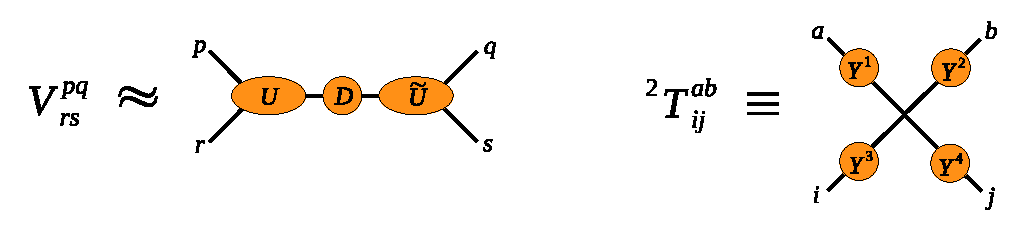
\includegraphics[width=0.9\textwidth]
{figures/cpd_rccsd/rccsd_cpd_def}}}
.
\label{fig:rccsd_cpd_def}
\end{equation}
%
Following the procedure described in Chapter~\ref{ch:tcc}, we derived 
an ALS-like update rule for the factors $Y \in \{Y^{1}, Y^{2}, Y^{3}, Y^{4}\}$. 
We call this method CPD-RCCSD. 
After defining proper intermediates with an automated algebraic 
system,\cite{drudge2} the cost of iteration in CPD-RCCSD is quartic in the 
basis size, auxiliary basis size and $r_{T}$.

CP decomposition was applied in the contest of RCCD before by Benedict and 
Auer\cite{benedict_ccd, benedict_mp2}. Although conceptually similar, our 
method significantly differs by the way one solves for the factors $Y$ of 
the ${}^2T$ amplitude and the use of standard RI decomposition of two electron 
integrals instead of CPD in the mentioned works.

To study the properties of this new method, we first apply it to weakly 
correlated problems used in the evaluation of 
THC-RCCSD.\cite{schutski2017tensor} Additionally, we show how our 
approximate CC methods work in strong correlation regime by simulating 
one dimensional Hubbard model\cite{essler2005one} and nitrogen 
dissociation.

\subsection{Computational details}
The CPD-RCCSD code is written in Python\cite{van2007python} on top of the 
PySCF\cite{sun2017python} electronic structure package. Hartree-Fock solutions, 
as well as two-electron integrals and density fitted integrals were 
provided by PySCF. For molecular systems we used standard cc-pVDZ basis set from 
the EMSL database,\cite{schuchardt2007basis} along with the cc-pVDZ-jkfit for 
RI decomposition. In case of Hubbard Hamiltonian~\ref{sec:hubbard_hamiltonian} 
the RI decomposition was built analytically.

For simulations of molecules in Table~\ref{tab:energies_cpd_rccsd} CC iterations 
were stopped after energy converged to within $10^{-6}~\mathrm{H}$ or a limit 
of 500 iterations was reached. In case of Hubbard Hamiltonian we used a 
threshold of $10^{-12}~\mathrm{H}$ for energy and 2000 iterations. The 
simulations presented in section~\ref{sec:strong_correlation} used up to 2000 
iterations, and $10^{-8}~\mathrm{H}$ convergence threshold. 

\subsection{CPD-RCCSD in weakly correlated systems}
To test the properties of CPD-RCCSD, we first apply it to weakly correlated 
Hubbard model (see Section~\ref{sec:hubbard_hamiltonian}). The convenience of 
the Hubbard Hamiltonian is that the two body interaction term in the on-site 
basis has simple structure. The full 4-index interaction in a model with $N$ 
sites is a diagonal tensor of size $N\times N\times N \times N$, having $\eta$ 
on the diagonal. Exact representations of the Hubbard interaction tensor in 
various forms can be easily built.

The exact RI representation ($V_{pqrs} = 
\eta \sum_{\alpha} U_{pr\alpha} \tilde{U}_{qs\alpha}$) of Hubbard interaction 
has rank $N$. Tree index RI factors can be chosen to be sparse $N 
\times N \times N$ tensors with elements $U_{ij\alpha} = \tilde{U}_{ij\alpha} 
= \delta_{i}^{\alpha} \delta_{j}^{\alpha} \cdot \sqrt{\eta}$. Likewise, an 
exact THC decomposition ($V_{pqrs} = \eta \sum_{\alpha \beta} W^{1}_{p\alpha} 
W^{2}_{r\alpha} X_{\alpha, \beta} W^{3}_{q\beta} W^{4}_{s\beta}$) has ranks 
equal $N$, and matrices $W \in \{W^{1}, W^{2}, W^{3}, W^{4}, X\}$ are identity 
matrices of size $N \times N$. The scalar $\eta$ can be absorbed into matrix 
$X$. Finally, an exact CP decomposition ($V_{pqrs} = \eta \sum_{\alpha} 
W^{1}_{p\alpha} W^{2}_{r\alpha} W^{3}_{q\alpha} W^{4}_{s\alpha}$) has rank $N$.
Factor matrices, as previously, are identities. Summarizing, all decompositions 
of the Hamiltonian considered in this work can be built exactly and have low 
ranks. The approximation, thus, affects only cluster amplitudes.

The energy of $6, 10, 14$ and $18$-site Hubbard model was 
calculated at $\eta = 2$.
%
\begin{figure}[!tb]
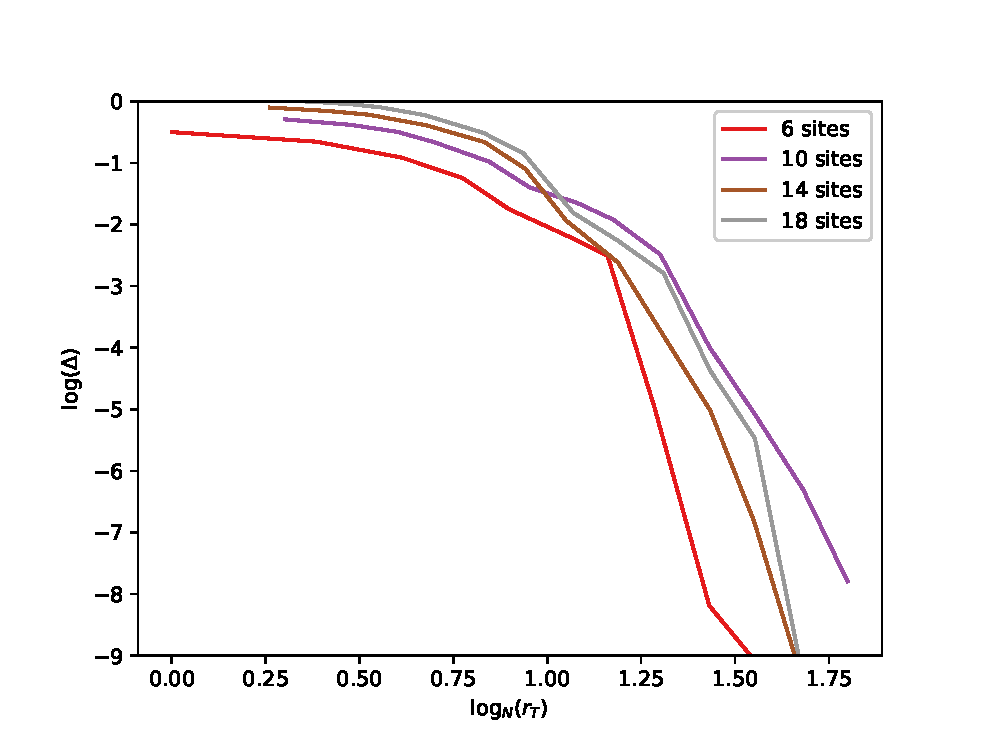
\includegraphics[width=\columnwidth]{figures/cpd_rccsd/err_vs_r_u_2_cpd}
\caption{Error in energy per site for Hubbard 
model at $\eta = 2$
\label{fig:err_vs_r_u_2}}
\end{figure}
%
As the graph demonstrates, the difference in the correlation energy 
between CPD-RCCSD and conventional RCCSD methods decays exponentially as the 
rank $r_{T}$ is increased, similarly to the THC-RCCSD method. At  
$r_{T} \sim N^{1.2} - N^{1.5}$ the difference induced by the decomposition 
of doubles amplitudes is less than $1 \textrm{mH}$, which an excellent 
approximation of RCCSD. 

To further assess the performance of CPD-RCCSD, we calculated he energy 
of a set of molecules, previously used for evaluating THC-RCCSD. The magnitude 
of $r_{T}$ is chosen to be a multiple of the size of the auxiliary basis used 
in the RI decomposition of the Hamiltonian.

\begin{center}
\begin{table}[!ht]
\caption{CCSD correlation energies ($E_c$), errors in
correlation energies ($\Delta E_c$)
and the norm of doubles residuals ($|{}^2R_{ij}^{ab}|$) for several small 
molecules.
\label{tab:energies_cpd_rccsd}}
\begin{tabular}{lccccccc}
\hline \hline
& & \multicolumn{2}{c}{$\Delta E_c~(mH)$} & 
\multicolumn{2}{c}{$|{}^2R_{ij}^{ab}|$}\\
\cline{3-4} \cline{5-6} System & $E_c~(mH)$ & $1.5 \, N_\mathrm{RI}$ &
$2 \, N_\mathrm{RI}$ & $1.5 \, N_\mathrm{RI}$ &
$2 \,~N_\mathrm{RI}$\\
\hline
AceticAcid & -228.506 & 5.955 & 3.169 & 0.262 & 0.195 \\
Aniline & -286.771 & 14.771 & 7.378 & 0.360 & 0.208 \\
Diboron tetrafluoride & -448.299 & 7.143 & 4.232 & 0.318 & 0.271 \\
Benzene & -231.559 & 11.144 & 5.596 & 0.298 & 0.167 \\
Butadiene & -155.525  & 4.717 & 2.483 & 0.198 & 0.105 \\
Cyclobutane & -156.738  & 5.215 & 2.329 & 0.185 & 0.094 \\
Dimethylsulfoxide & -552.232  & 5.206 & 2.518 & 0.221 & 0.149 \\
Furan & -229.390 & 9.540 & 4.675 & 0.310 & 0.191 \\
Isobutane & -157.973 & 4.187 & 2.242 & 0.124 & 0.087 \\
Methylformate & -228.479 & 6.247 & 3.271 & 0.267 & 0.198 \\
Methylnitrite & -244.398 & 7.112 & 3.856 & 0.290 & 0.209 \\
Pyridine & -247.570 & 11.996 & 6.341 & 0.311 & 0.205 \\
Pyrrole & -209.566 & 9.330 & 4.569 & 0.293 & 0.163 \\
Thiophene & -552.031 & 7.703 & 4.127 & 0.238 & 0.147 \\
Phenol & -306.608 & 14.430 & 7.419 & 0.366 & 0.224 \\
Toluene & -270.758 & 14.333 & 6.706 & 0.355 & 0.171 \\
mean unsigned error & & 8.689 & 4.432 & & &\\
max unsigned error & & 14.771 & 7.419 & & &\\
root-mean-square error& & 9.379 & 4.758 & & &\\
\hline\hline
\end{tabular}
\end{table}
\end{center}

The results in Table~\ref{tab:energies_cpd_rccsd} are similar to the results
of THC-RCCSD. As the rank $r_{T}$ is increased, the quality of approximation 
improves. Typical errors are around $5 mH$ for the rank of CPD of doubles 
amplitudes being twice bigger than the size of the auxiliary basis used in the 
decomposition of the Hamiltonian. The errors in CPD-RCCSD are around five times 
higher than in THC-RCCSD for the same rank values. We attribute this to the 
larger number of the parameters in THC-RCCSD, having $4 \cdot N r_{T} + 
r^{2}_{T}$ for parameterizing amplitudes versus $4 \cdot N r_{T}$ in CPD-RCCSD. 
The comparison of Tables~\ref{tab:energies_cpd_rccsd} and 
\ref{tab:energies_cpd_rccsd} shows, however, that the accuracy of CPD-RCCSD 
increases more monotonically with the size of the rank. We suspect that a 
cancellation of errors happens in case of THC-RCCSD because of the more 
complicated approximation to the Hamiltonian, and thous CPD-based coupled 
cluster provides a more predictable approximation.

\subsection{Conclusions}
To summarize, CPD-RCCSD provides an alternative efficient approximation to the 
coupled cluster with singles and doubles. Overall, CPD-RCCSD and THC-RCCSD 
have a similar accuracy and asymptotic scaling of computational cost. 
Practically, CPD-RCCSD is much faster due to the use of an efficient RI 
decomposition of the electron interaction in place of THC. Additional benefit 
of using canonical decomposition of amplitudes is that the method can be 
further generalized to higher order coupled cluster theories.


\section{Tensor structured CC in the strong correlation limit
\label{sec:strong_correlation}}
\subsection{Introduction}
In this section we will discuss the behavior of tensor structured CC methods 
in the strong correlation regime, as well as some possible future lines of 
research. As was mentioned in Chapter~\ref{ch:introduction}, strong correlation 
presents a major challenge to current many-body methods. Standard 
coupled cluster methods perform poorly for strong correlation, unless allowed 
to break proper physical symmetries of the wavefunction or very high orders of 
excitation operators are taken into account. Both of the latter options are 
implausible in applications.

The simplest case when strong correlation arises in molecular systems is the 
dissociation of multielectron bonds and various transition state 
configurations. Model Hamiltonians are also a convenient benchmark for 
many-body methods in strong correlation. The eigenstates of the Hubbard 
Hamiltonian at half-filling are strongly correlated when the on-site repulsion 
is significantly higher than the kinetic energy, e.g. $\eta = U / t \gg 0$. We 
used these two settings to test the behavior of tensor structured coupled 
cluster methods.

\subsection{Rank restriction in TCC at strong correlation}
All coupled cluster calculations in this section used up to 2000 iterations and 
$10^{-8}$ convergence threshold. Other parameters were chosen in the same 
way as described in Sections~\ref{sec:thc_rccsd} and~\ref{sec:cpd_rccsd}. 

As a first test, we applied CPD-RCCSD to Hubbard models with $6$, $10$ and $14$ 
sites. 
%
\begin{figure}[ht!]
\centering
%\begin{subfigure}{0.75\textwidth}
%\centering
%\includegraphics[width=1\linewidth]
%{figures/tcc_strong_correlation/energy_vs_u_6_sites_cpd_rccsd}
%\caption{6 sites}
%\label{fig:energy_vs_u_6_sites_cpd_rccsd}
%\end{subfigure}
%\begin{subfigure}{0.75\textwidth}
%\centering
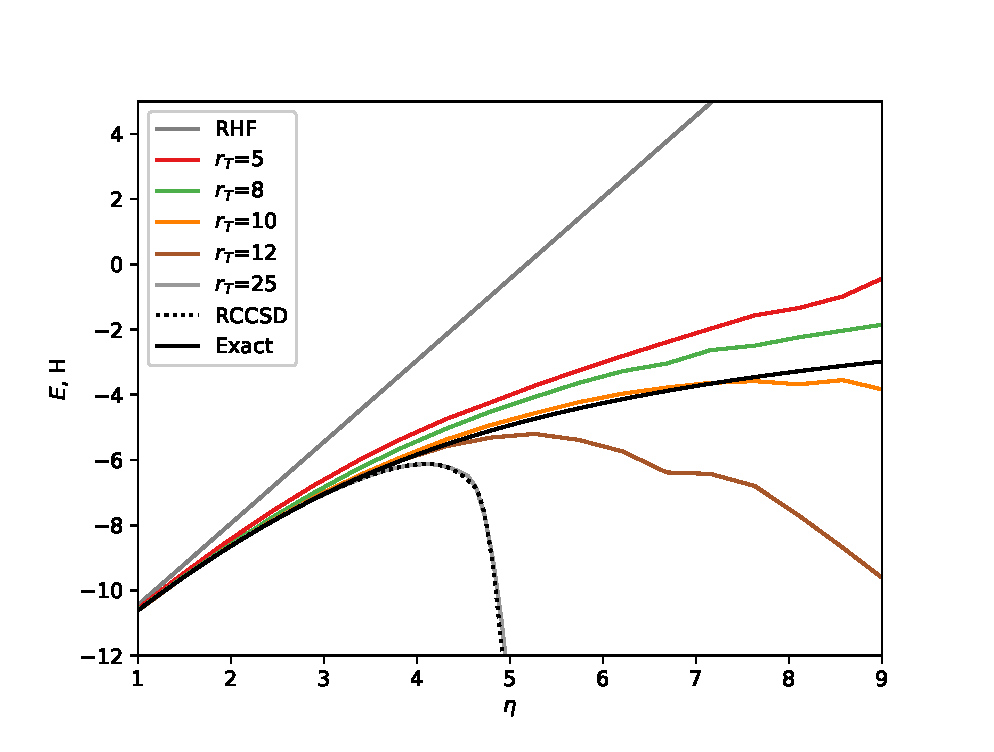
\includegraphics[width=\columnwidth]
{figures/tcc_strong_correlation/energy_vs_u_10_sites_cpd_rccsd}
%\caption{10 sites}
%\label{fig:energy_vs_u_10_sites_cpd_rccsd}
%\end{subfigure}
\caption{Energy behavior for different ranks of CP decomposition of amplitudes. 
Hubbard model at half-filling, 10 sites}
\label{fig:energy_vs_u_cpd}
\end{figure}
%
Figure~\ref{fig:energy_vs_u_cpd} shows the dependence of the total energy 
on the interaction strength $\eta$. As expected, conventional RCCSD provides 
a good description of Hubbard rings at low $\eta$, and systematically 
overestimates the energy as the system becomes strongly correlated. CPD-RCCSD, 
however, demonstrates a surprising effect. If one chooses the approximation to 
the doubles amplitudes to be the low 
rank, the incorrect behavior of the original RCCSD method may be fixed. As the 
rank is increased, the solutions of CPD-RCCSD gradually change behavior between 
the Hartree-Fock (no correlation) and conventional RCCSD 
(overestimation of correlation energy), as can be seen on 
Figure~\ref{fig:energy_vs_u_cpd}. This situation, however, is not 
specific to CPD-RCCSD, and is also observed with THC-RCCSD (see 
Figure~\ref{fig:energy_vs_u_thc}).
%
\begin{figure}[ht!]
\centering
%\begin{subfigure}{0.75\textwidth}
%\centering
%\includegraphics[width=1\linewidth]
%{figures/tcc_strong_correlation/energy_vs_u_6_sites_thc_rccsd}
%\caption{6 sites}
%\label{fig:energy_vs_u_6_sites_thc_rccsd}
%\end{subfigure}
%\begin{subfigure}{0.75\textwidth}
%\centering
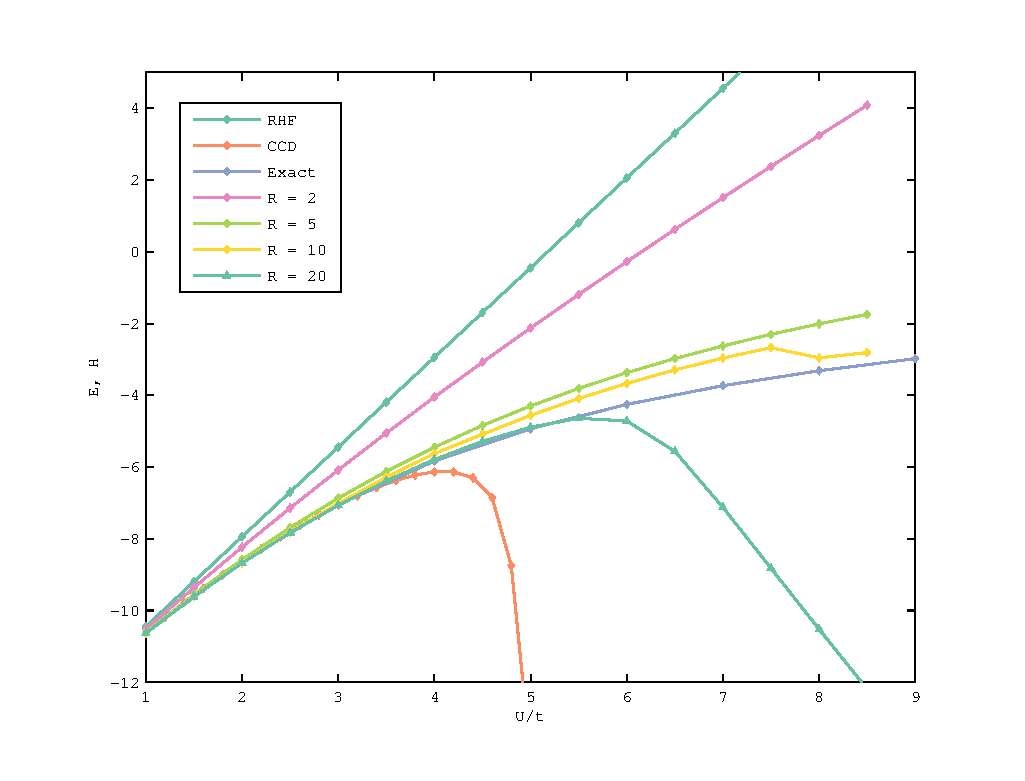
\includegraphics[width=\columnwidth]
{figures/tcc_strong_correlation/energy_vs_u_10_sites_thc_rccsd}
%\caption{10 sites}
%\label{fig:energy_vs_u_10_sites_thc_rccsd}
%\end{subfigure}
\caption{Energy behavior for different ranks of THC decomposition of 
amplitudes. Hubbard model at half-filling, 10 sites}
\label{fig:energy_vs_u_thc}
\end{figure}
%
The difference in the case of THC-RCCSD is that the overcorrelation happens at 
slightly larger ranks (compare, for example, $r_{T} = 5$ and $r_{T} = 10$ 
between Figures~\ref{fig:energy_vs_u_cpd} and \ref{fig:energy_vs_u_thc}). Both 
methods, however, reproduce standard RCCSD when sufficiently large ranks of the 
decompositions are chosen, as one may expect.

The results observed with the Hubbard Hamiltonian do not change qualitatively 
in the case of molecular systems. Figure~\ref{fig:energy_vs_d_cc-pvdz} 
demonstrates the effect of rank restriction in CPD-RCCSD for the calculation of 
the dissociation curve of nitrogen. With rank equal 4, the solution has the 
correct behavior at the dissociation limit, while for larger ranks CPD-RCCSD 
approximates standard RCCSD. The rank restricted solutions, however, miss a 
fair amount of weak correlation energy, which plays a major role in molecular 
systems (near the equilibrium exact and 
CPD-RCCSD curves are far apart). Having seen the behavior of rank restricted 
approximate coupled cluster for a wide range of systems, we would like to 
provide an interpretation of the observed effect.
%
\begin{figure}[!ht]
\centering
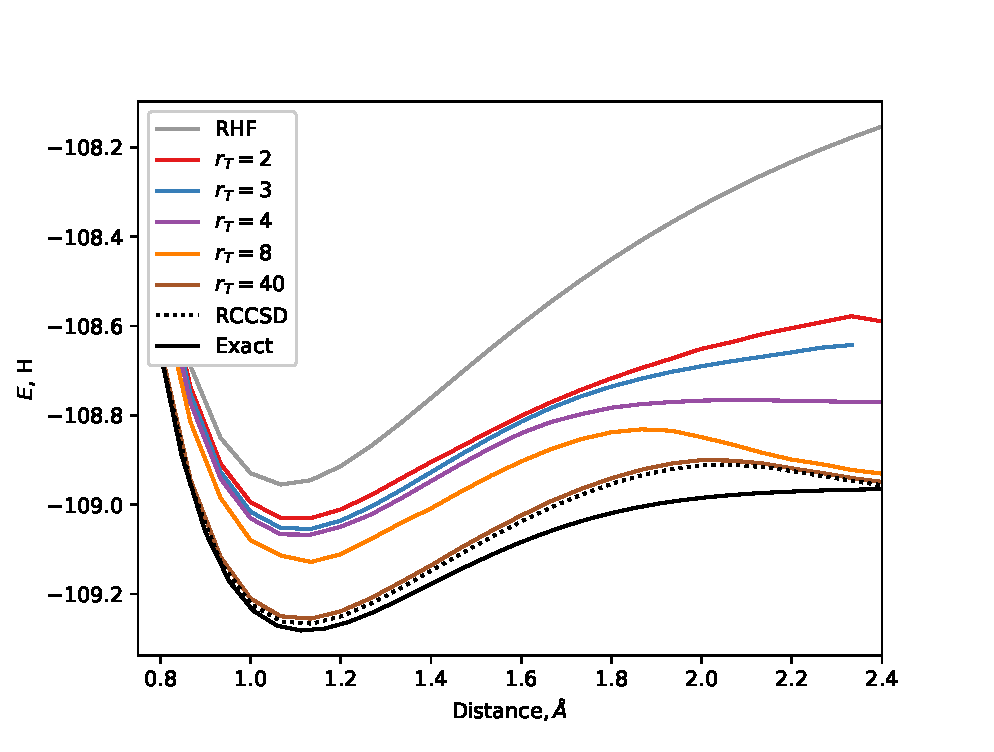
\includegraphics[width=\columnwidth]
{figures/tcc_strong_correlation/energy_vs_d_cc-pvdz}
\caption{Energy behavior for different ranks of CP decomposition of 
amplitudes. Dissociation of nitrogen, cc-pVDZ}
\label{fig:energy_vs_d_cc-pvdz}
\end{figure}
%

\subsection{Tentative explanation}
Let us offer a tentative explanation of the observed effect based on additional 
parameters of the rank-restricted solutions. As was noted before, at strong 
correlation several configurations become degenerate and this degeneracy 
is caused by physical symmetries encoded in the 
Hamiltonian.\cite{scuseria2011projected,jimenez2012projected} Some of the 
entries of excitation operators, which correspond to degenerate configurations, 
have to get larger and larger values. We argue that this imbalance, namely a 
significantly higher importance of a small subset of amplitudes over the rest of 
them, is what makes residual equations in coupled cluster an ill-posed problem. 
This may be paralleled to solving an overdetermined nonlinear system.

Degroote~\emph{et al.}~\cite{degroote2016polynomial} demonstrated
that in the strong correlation regime cluster amplitude tensors may factorize, 
e.g. that the effective number of parameters in cluster amplitudes is lower. 
The later is the idea behind their polynomial similarity transformation theory, 
which uses general polynomial series instead of an exponent to parameterize 
the wavefunction. The non-exponential similarity transformation leads to a 
different set of residual equations, where dominant amplitudes have larger 
contributions to the residual. The amplitudes in these CC-like methods do not 
grow to large values, in contrast with traditional coupled cluster.
A similar situation is observed with rank-restricted solutions in our approach.

%
\begin{figure}[ht]
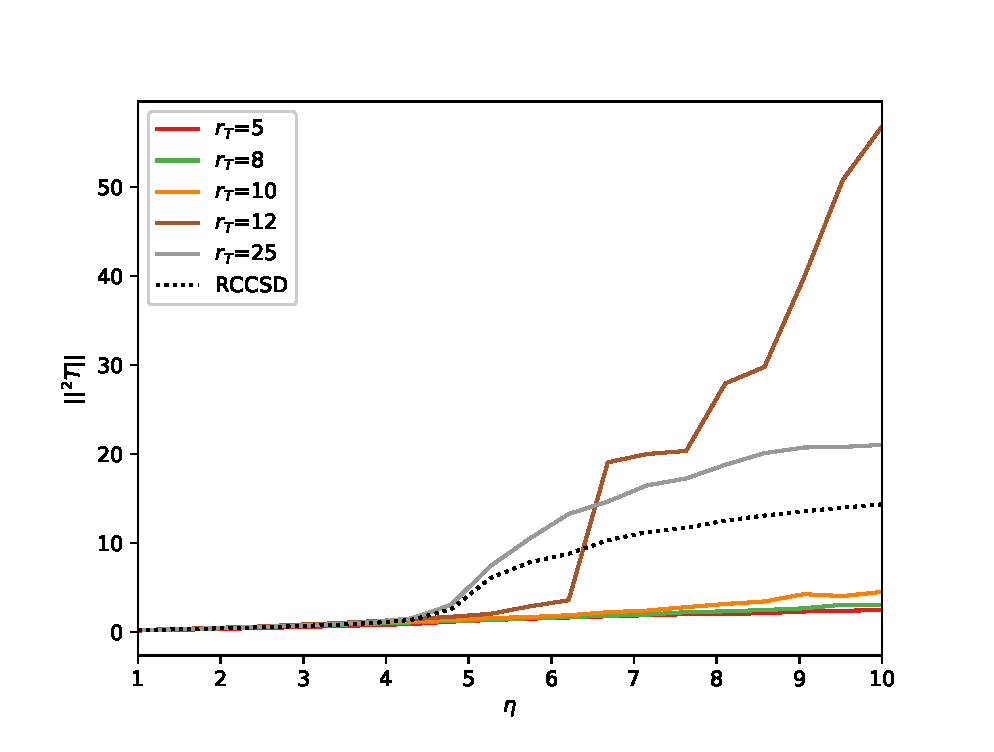
\includegraphics[width=\columnwidth]
{figures/tcc_strong_correlation/t2_norms_vs_u_10_sites_cpd_rccsd}
\caption{Frobenius norm of ~ ${}^2T$ amplitudes for different ranks $r_{T}$ in 
CPD-RCCSD 
calculations. Hubbard model at half-filling, 10 sites.
\label{fig:t2_norms_vs_u_10_sites_cpd_rccsd}}
\end{figure}
%
In Figure~\ref{fig:t2_norms_vs_u_10_sites_cpd_rccsd} the dependence of the norm 
of the ${}^2T$ amplitudes as a function of rank and on-site repulsion is shown. 
As the graph illustrates, the norm of the doubles amplitudes in the physically 
proper-behaving low rank solutions is lower than the norm of ${}^2T$ amplitudes 
in conventional RCCSD. In contrast, as the ranks grow and CPD-RCCSD starts 
to overcorrelate, there is a sharp increase in the amplitude norm to values 
even higher than the standard RCCSD would yield. For example, the solution with 
$r_{T} = 12$, which significantly overcorrelates at $\eta > 6$ (see 
Figure~\ref{fig:energy_vs_u_cpd}, yellow line) also has large 
norm of ${}^2T$ amplitudes starting at the same values of $\eta$ 
(Figure~\ref{fig:t2_norms_vs_u_10_sites_cpd_rccsd}, yellow line). 

Moreover, the low-rank solutions in tensor structured CC 
do not satisfy the standard residual equations in analogy to the CC-like 
method of Degroote~\emph{et al.} we mentioned.
Figure~\ref{fig:r2_norms_vs_u_10_sites_cpd_rccsd} demonstrates the 
dependence of the residual norm on the correlation strength parameter $\eta$ 
for different ranks. The physically well behaving cluster amplitudes deviate 
from being the solutions of the residual equations as $\eta$ increases.
The individual factors in the decomposition of amplitudes, however, \emph{do} 
satisfy their own ALS-like equations (see Chapter~\ref{ch:tcc}). The CC 
residuals are large for low-rank solutions and sharply drop as 
CPD-RCCSD amplitudes approach regular RCCSD amplitudes as one may 
expect (compare $r_{T} = 8$ 
and $r_{T} = 25$ in 
Figures~\ref{fig:energy_vs_u_thc},~\ref{fig:t2_norms_vs_u_10_sites_cpd_rccsd} 
and~\ref{fig:r2_norms_vs_u_10_sites_cpd_rccsd}). 
%
\begin{figure}[ht]
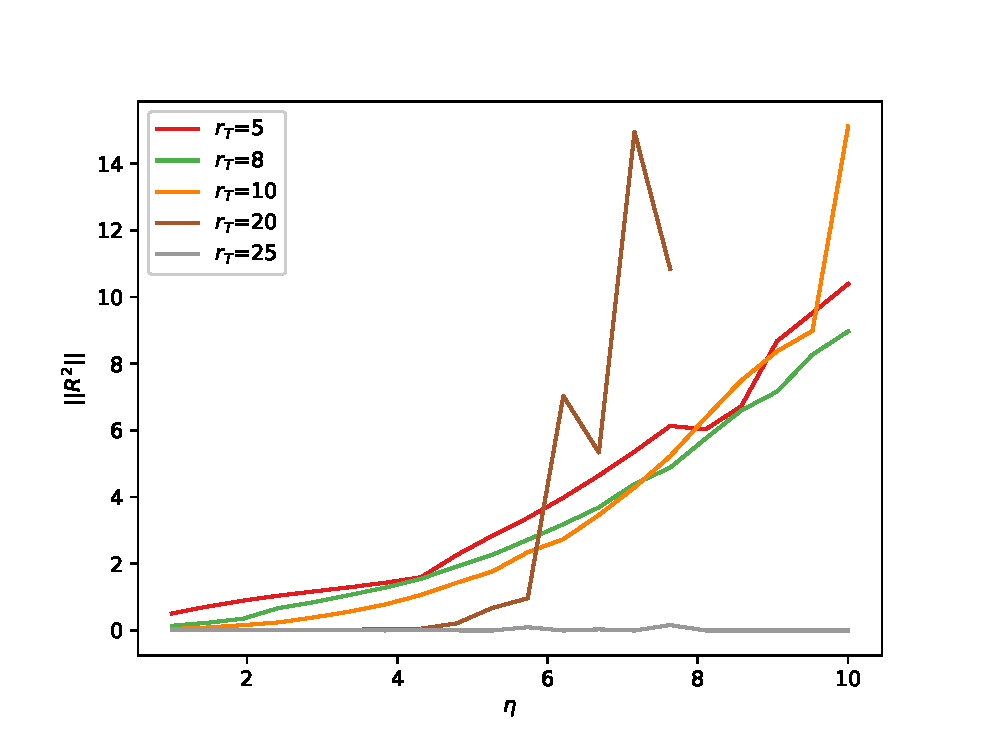
\includegraphics[width=\columnwidth]
{figures/tcc_strong_correlation/r2_norms_vs_u_10_sites_cpd_rccsd}
\caption{Frobenius norm of ~${}^2T$ residuals for different ranks $r_{T}$ in 
CPD-RCCSD 
calculations. Hubbard model at half-filling, 10 sites}
\label{fig:r2_norms_vs_u_10_sites_cpd_rccsd}
\end{figure}
%
To summarize our observations, rank restriction of the 
amplitudes seems to be a way to regularize conventional CC equations 
in strong correlation regime. We would like to point out that similar 
regularization schemes (called "dropout regularization") are ubiquitous in 
machine learning literature.~\cite{srivastava2014dropout, wan2013regularization} 
This raises a question whether other regularization techniques, like 
standard $l_{2}$-norm regularization,\cite{tikhonov1963solution} can be applied 
in the coupled cluster method.

Let us mention last that the idea of Degroote~\emph{et 
al.}~\cite{degroote2016polynomial} was further developed in our group in a 
series of publications~\cite{degroote2016polynomial, gomez2017attenuated, 
qiu2017projected2, hermes2017combining}. In these works different 
similarity transformations were developed for specific model Hamiltonians. While 
being highly efficient both at strong and weak correlation regimes, these
CC-like methods use different ansatze for each symmetry responsible for 
the onset of strong correlation. The search for a universal approach for
strongly correlated systems thus still continues.

\subsection{Conclusions}
The strong correlation regime poses a hard problem for most many-body methods. 
Coupled cluster methods, while being very effective for weakly correlated 
systems, fail when strong correlation dominates. Recently a series of 
promising CC-like theories was developed in our 
group.\cite{degroote2016polynomial, gomez2017attenuated, 
qiu2017projected2, hermes2017combining} 
The problem of these theories, however, is that the explicit form of equations 
depends on the symmetry of the Hamiltonian responsible for the onset of strong 
correlation, and the idea is hard to generalize for arbitrary Hamiltonians. On 
the other hand, rank restriction in tensor structured CC provides a alternative 
way to regularize the solutions of standard coupled cluster at strong 
correlation, independently of the form of the Hamiltonian. More research is 
needed to make this approach practically applicable, but we believe the idea 
may be interesting in future method development.
\chapter{Conclusions and outlook
\label{ch:conclusions}}
In this work, two new approximate coupled cluster methods were developed. Our 
approach is based on tensor decompositions, which are alternative 
representations of high-dimensional tensors ubiquitous in post-Hartree-Fock 
theories. After an introduction into the theory of coupled cluster, we 
focus on three tensor formats employed in this work: resolution of 
identity (RI), canonical polyadic decomposition (CPD) and tensor 
hypercontraction (THC). We represent these tensor formats in a uniform way 
with the help of tensor diagrams and discuss techniques to cast different 
index-based tensors into CPD and THC forms. 

When higher-order tensors are approximated with tensor decompositions, the 
decisive quantity is the length of the expansion (the rank). The cost of 
tensor contractions with decomposed tensors depends on the form of the 
decomposition, the rank(s) $r$ and the basis size $N$. We 
demonstrate that intermediates in coupled cluster can be calculated at 
cost scaling as the 4th power of $r$ and $N$. The discussion culminates by 
the derivation of a general tensor-structured coupled cluster method using THC 
factorization as an example. In our approach the Alternating Least Squares 
procedure is combined with the coupled cluster update to produce a new 
iterative algorithm for the factors of the decomposed cluster amplitudes. This 
generic algorithm has quartic cost per iteration if the THC or the CPD 
factorization is used for the amplitude tensors.

After establishing a general framework for tensor structured coupled cluster, 
we present its first concrete realization, namely THC-RCCSD. We demonstrate 
that only small ranks of order $N^{1.3}$ in the THC decomposition of 
the two-body interaction are sufficient for sub-mHartree accuracy in the MP2 
energy, and that the quality of the decomposition does not depend significantly 
on the choice of the basis. After combining the THC factorized two-body 
interaction with THC factorized amplitudes, we demonstrate that only small ranks 
of order $N^{1.3}$ are needed for the sub-mHartree accuracy of the resulting 
THC-RCCSD method. Given these findings, the overall scaling of THC-RCCSD is 
of order 
$O(N^{5})$ for sub-mHartree accuracy, whereas the original RCCSD method has 
$O(N^{6})$ computational cost. The method is tested on a large set of organic 
molecules.   

We then introduce another combination of tensor decompositions to approximate 
RCCSD. The two-body interaction is represented in a standard RI form, 
while the cluster amplitudes are treated in CPD format. The resulting CPD-RCCSD 
procedure again has a quartic cost in the ranks and basis, but is 
superior to the THC-based method due to the use of the fast RI factorization. We 
prove that sub-mHartree accuracy is obtained with ranks of order 
$O(N^{1.3})$, and hence the overall cost of CPD-RCCSD is similar to THC-RCCSD. 
We found that the error of CPD-RCCSD is around $5$ times larger than that of 
the THC-based method with the same rank, but the number of parameters is much 
less and scales only linearly with rank and $N$. Overall, CPD-RCCSD presents a 
faster and simpler alternative to THC-RCCSD. 

Finally, we have demonstrated that the failure of coupled cluster in the strong 
correlation regime can be mitigated by using low-rank decompositions of 
cluster amplitudes. We argue that low-rank approximations provide a way to 
regularize ill-posed residual equations and draw analogies to methods 
motivated by similar ideas. The latter provides a direction for future 
research.

As the framework we developed is quite general, many extensions are possible. 
Tensor-structured coupled cluster can be directly applied to unrestricted or 
generalized coupled cluster theories. These methods work better for strongly 
correlated molecular systems at the expense of breaking the spin symmetry of 
the wavefunction. CPD-RCCSD can be directly generalized to higher orders of 
coupled cluster theory, for example CCSDT, CCSDTQ, CCSDTQ5, where much larger 
numerical savings may be obtained. Additionally, the techniques we describe 
can be used in other CC-like approaches, such as the polynomial 
similarity transformation methods.\cite{degroote2016polynomial, 
gomez2017attenuated} Finally, the regularizing effect of 
low-rank amplitudes calls for the study of regularization methods in the 
coupled cluster approach.
\appendix

%\include{append-a}
%\appendix
%\addcontentsline{toc} {chapter}{\numberline {}Appendix A}  
%\include{append-a}
%\include{append-b}
%\addcontentsline{toc} {chapter}{\numberline {}Bibliography}{}
%\include{biblio}

\bibliographystyle{ieeetr}
\bibliography{references}
\end{document}
